\section{Re-calibration after ProtoDUNE-SP operation}
\label{sec:new_calib}

\noindent After the decommissioning of ProtoDUNE-SP in 2020, the temperature sensors were disconnected from the TGM and re-calibrated multiple times (see Table \ref{tab:calib}), using both LAr and LN2 as cryogenic media. Two sensors were damaged during the decommissioning process and were not replaced until the LAr-2023 calibration campaign. The comparative analysis of those re-calibrations not only offers insights into the long-term stability of the sensors but also elucidates any potential dependencies on the choice of the cryogenic liquid. Although DUNE will use LAr, massive RTD calibration would benefit from using LN2, given its higher accessibility and lower cost.

\begin{table}[htbp]
\begin{center}
\begin{tabular}{l c c}
Date & Cryogenic liquid & \# Sensors in capsule  \\ \hline
March 2018     &   LAr    &  4  \\
February 2022  &   LN2    & 14  \\
March 2023     &   LN2    & 14  \\
July 2023      &   LAr    & 14  \\
\end{tabular}
\end{center}
\caption{Calibration runs with indication of the date, the cryogenic liquid used and the number of sensors inside the capsule.}
\label{tab:calib}
\end{table}

In this section, a description of the setup used for these new calibrations, the changes applied to the procedure as well as the results and conclusions of these calibrations are presented.

%--------------------------------------------------------
\subsection{Evolution of the calibration setup}
\label{sec:new_calib_setup}

\noindent The FD-HD module will be equipped with over 500 precision sensors~\cite{dune_tdr4}, making the use of the current calibration setup impractical, as it can accommodate only four sensors simultaneously. Significant modifications have been introduced in order to increase this number to twelve, while maintaining the precision achieved during the 2018 calibration campaign. This was accomplished by positioning sensors at the same height, to avoid any potential vertical gradient, and following a cylindrical configuration, under the assumption that convection inside the capsule has rotational symmetry.
This symmetry is also kept outside the capsule in all concentric cryogenic containers, having added a fourth independent volume which should further reduce convection inside the inner capsule.
This notable advancement greatly streamlines the calibration process and serves to reduce both statistical and systematic errors associated with the procedure. Fig. \ref{fig:newSetup} shows the different elements of the new calibration setup, which are described below:

\begin{itemize}
    \item A polystyrene box with dimensions $55\times35\times30$ cm$^{3}$ and $4.5$ cm thick walls with a dedicated cover of the same material.
    \item Extruded polystyrene rectangles with a cylindrical hole of $12.5$ cm diameter and $25$ cm height, to conform the inner volume.
    \item A PTFE container with $12.5$ cm diameter, $25$ cm height and $2$ mm thick walls to fit in the hole left in the box. The approximate volume is $2$ L.
    \item A 3D printed PLA cylinder with two independent concentric volumes, placed inside the PTFE container.
    \item A cylindrical aluminum capsule to be placed in the inner volume of the PLA cylinder. It has $7$ cm diameter,  $14$ cm height and $1$ mm thick walls.
    \item A 3D printed PLA holder for 14 sensors, 12 of them forming a circle (the `corona') and the other 2 at the center, to be used as references. This support can be attached to the aluminum capsule at a fixed height. Cables are naturally extracted from the top of the assembly. A detailed view of this holder can be found in Fig. \ref{fig:newSetup}.
    \item The readout electronics, described in Sec.~\ref{sec:readout} has been retained from the previous setup.
    \item A more cost effective cable with similar performance has been used. Produced by Tempsens \cite{tempsens}, it has four twisted cables instead of two separated twisted pairs and an additional Kapton insulation layer between the shielding mesh and the four conductors. Its diameter is 2.7 mm.
\end{itemize}

\begin{figure}[htbp]
\centering
%{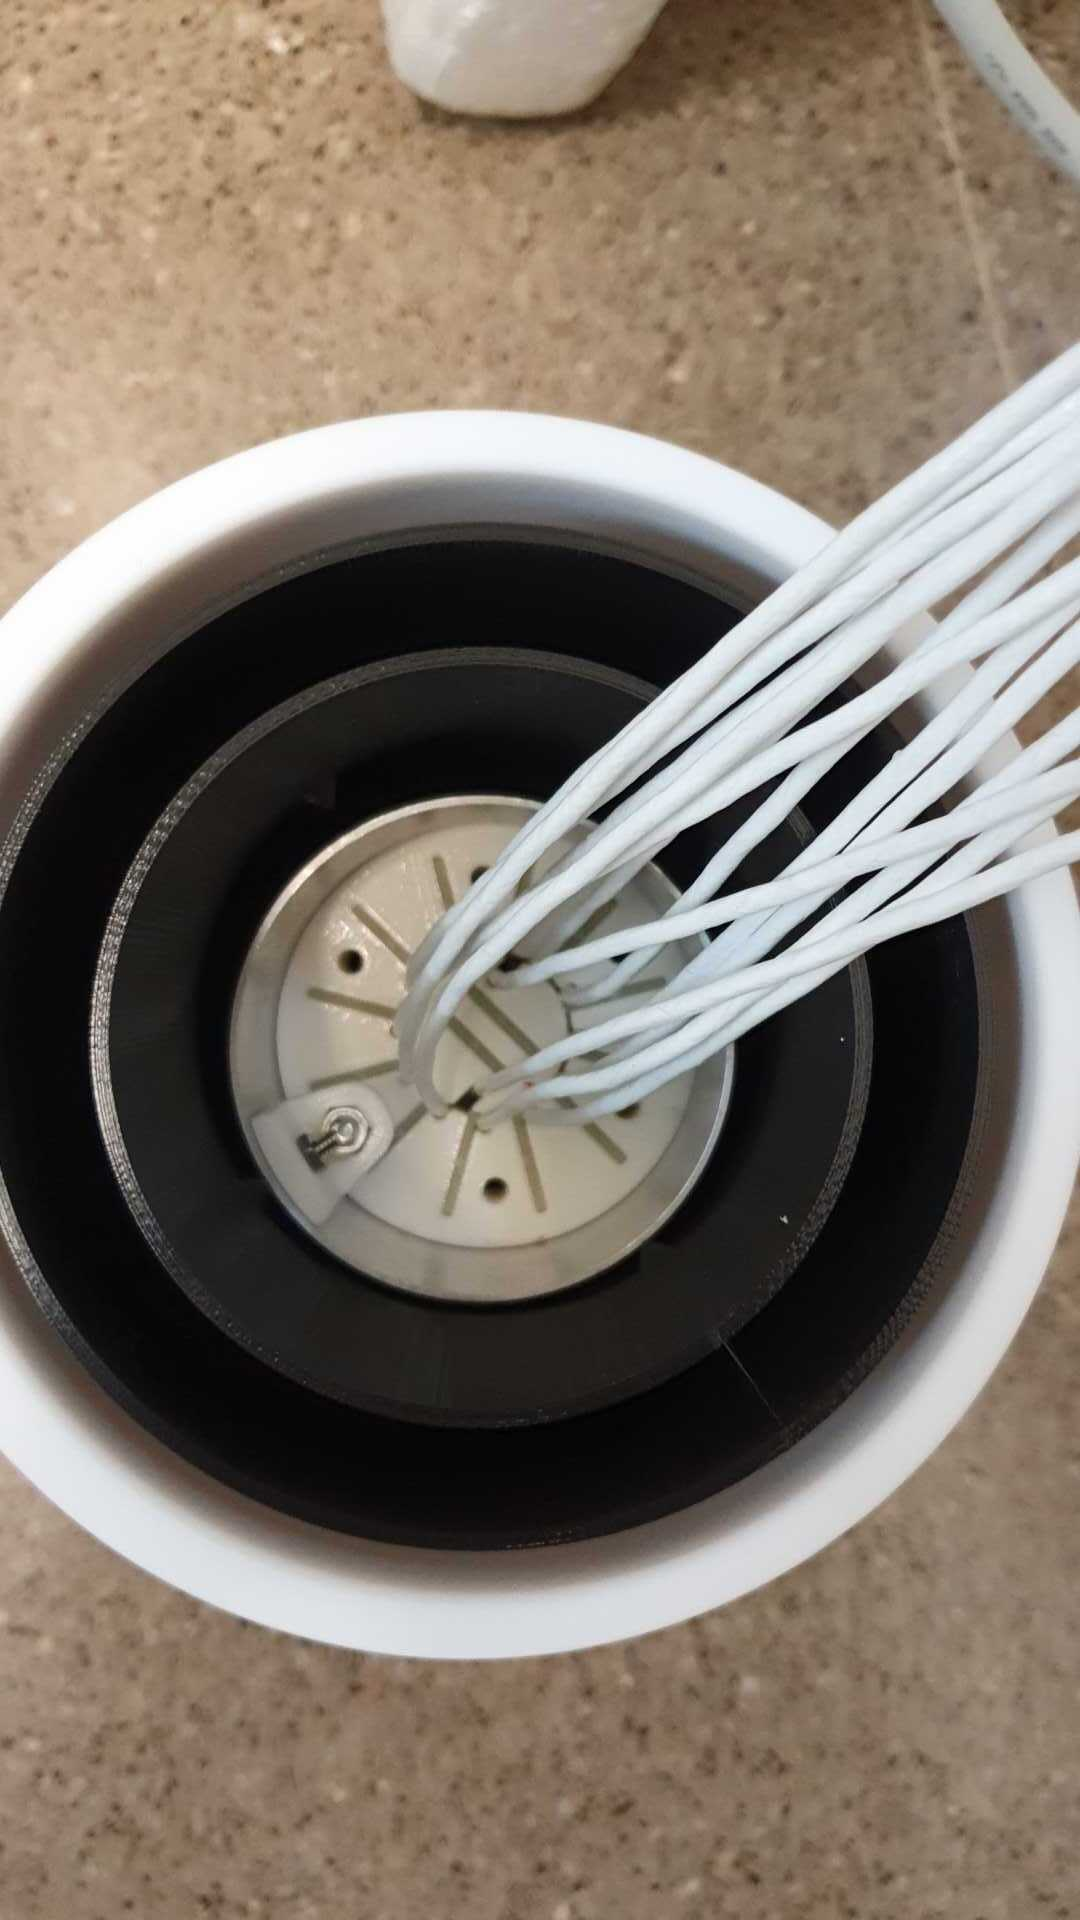
\includegraphics[width=0.303\textwidth,
%trim=0cm 4cm 0cm 4.7cm, clip]{images/figure_16_a.jpg}}
%{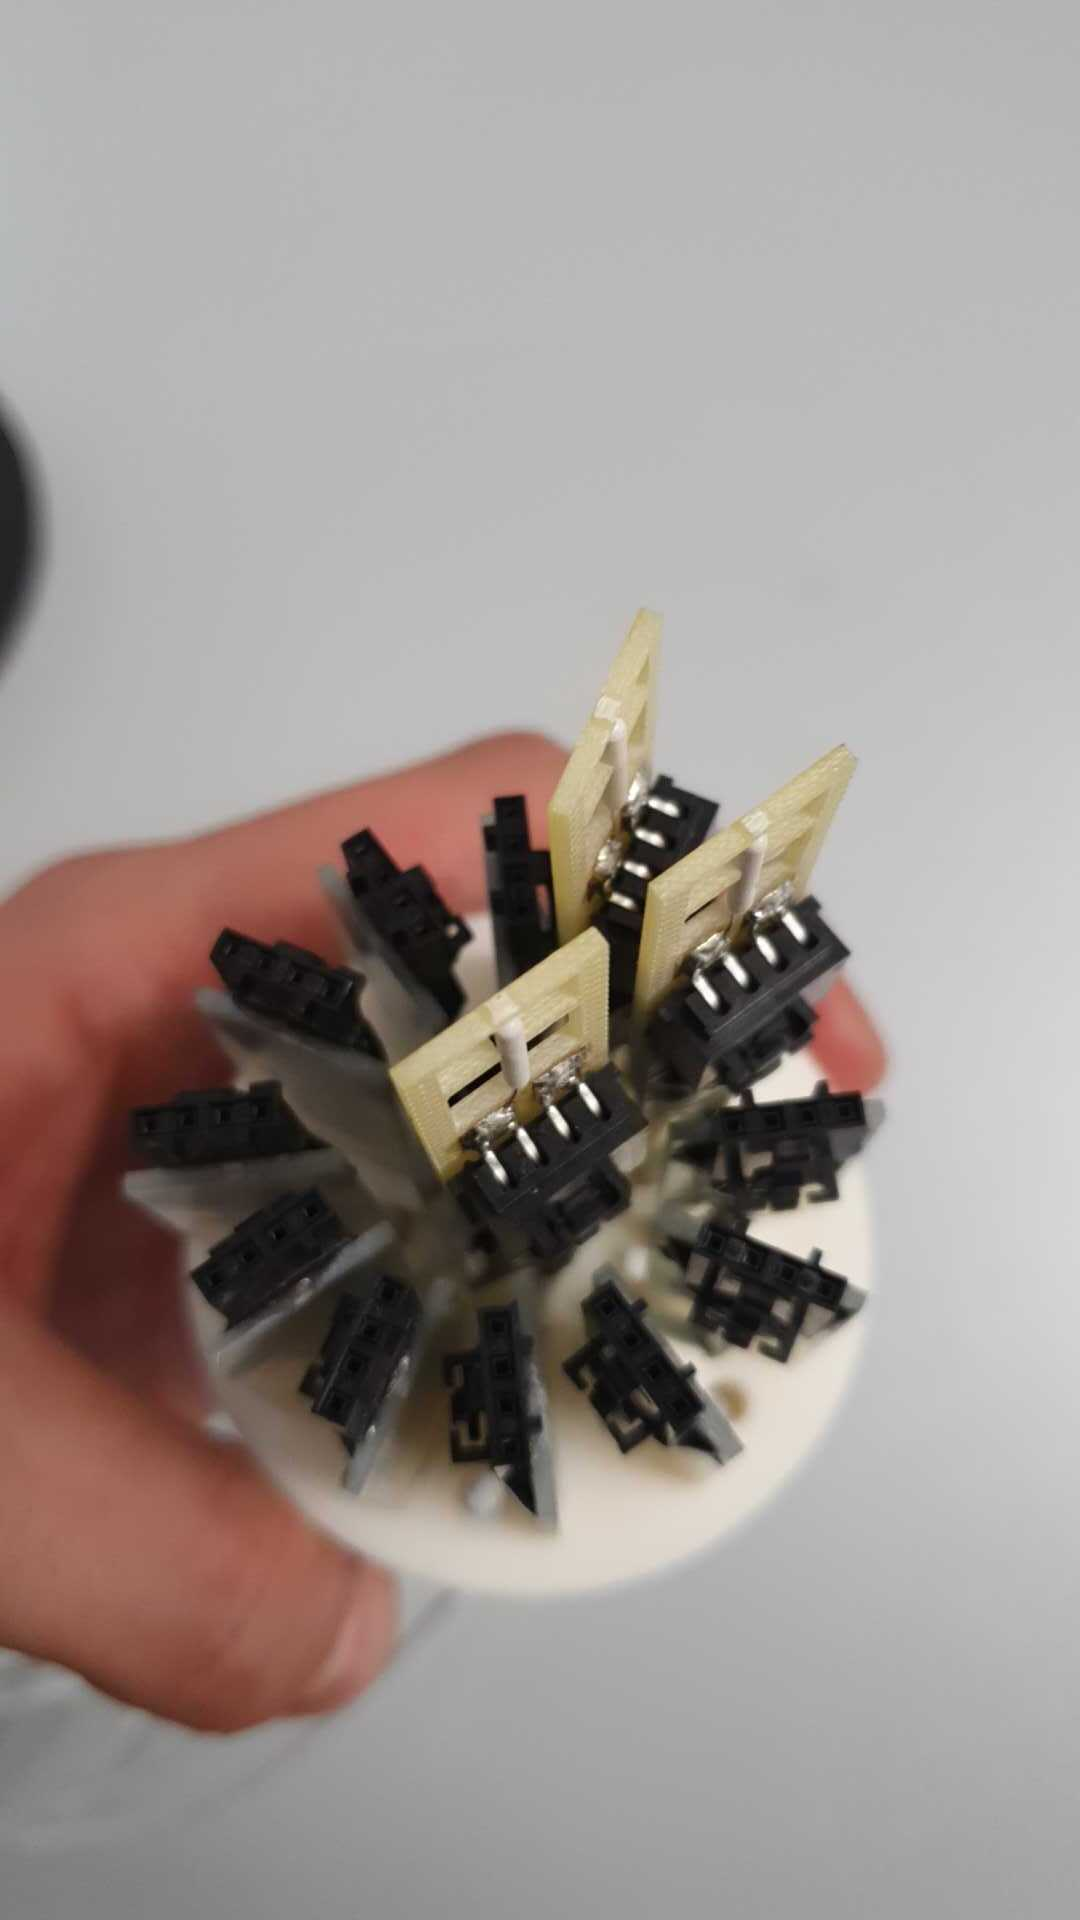
\includegraphics[width=0.3\textwidth, trim=0cm 4cm 0cm 7cm, clip]{images/figure_16_b.jpg}}
%{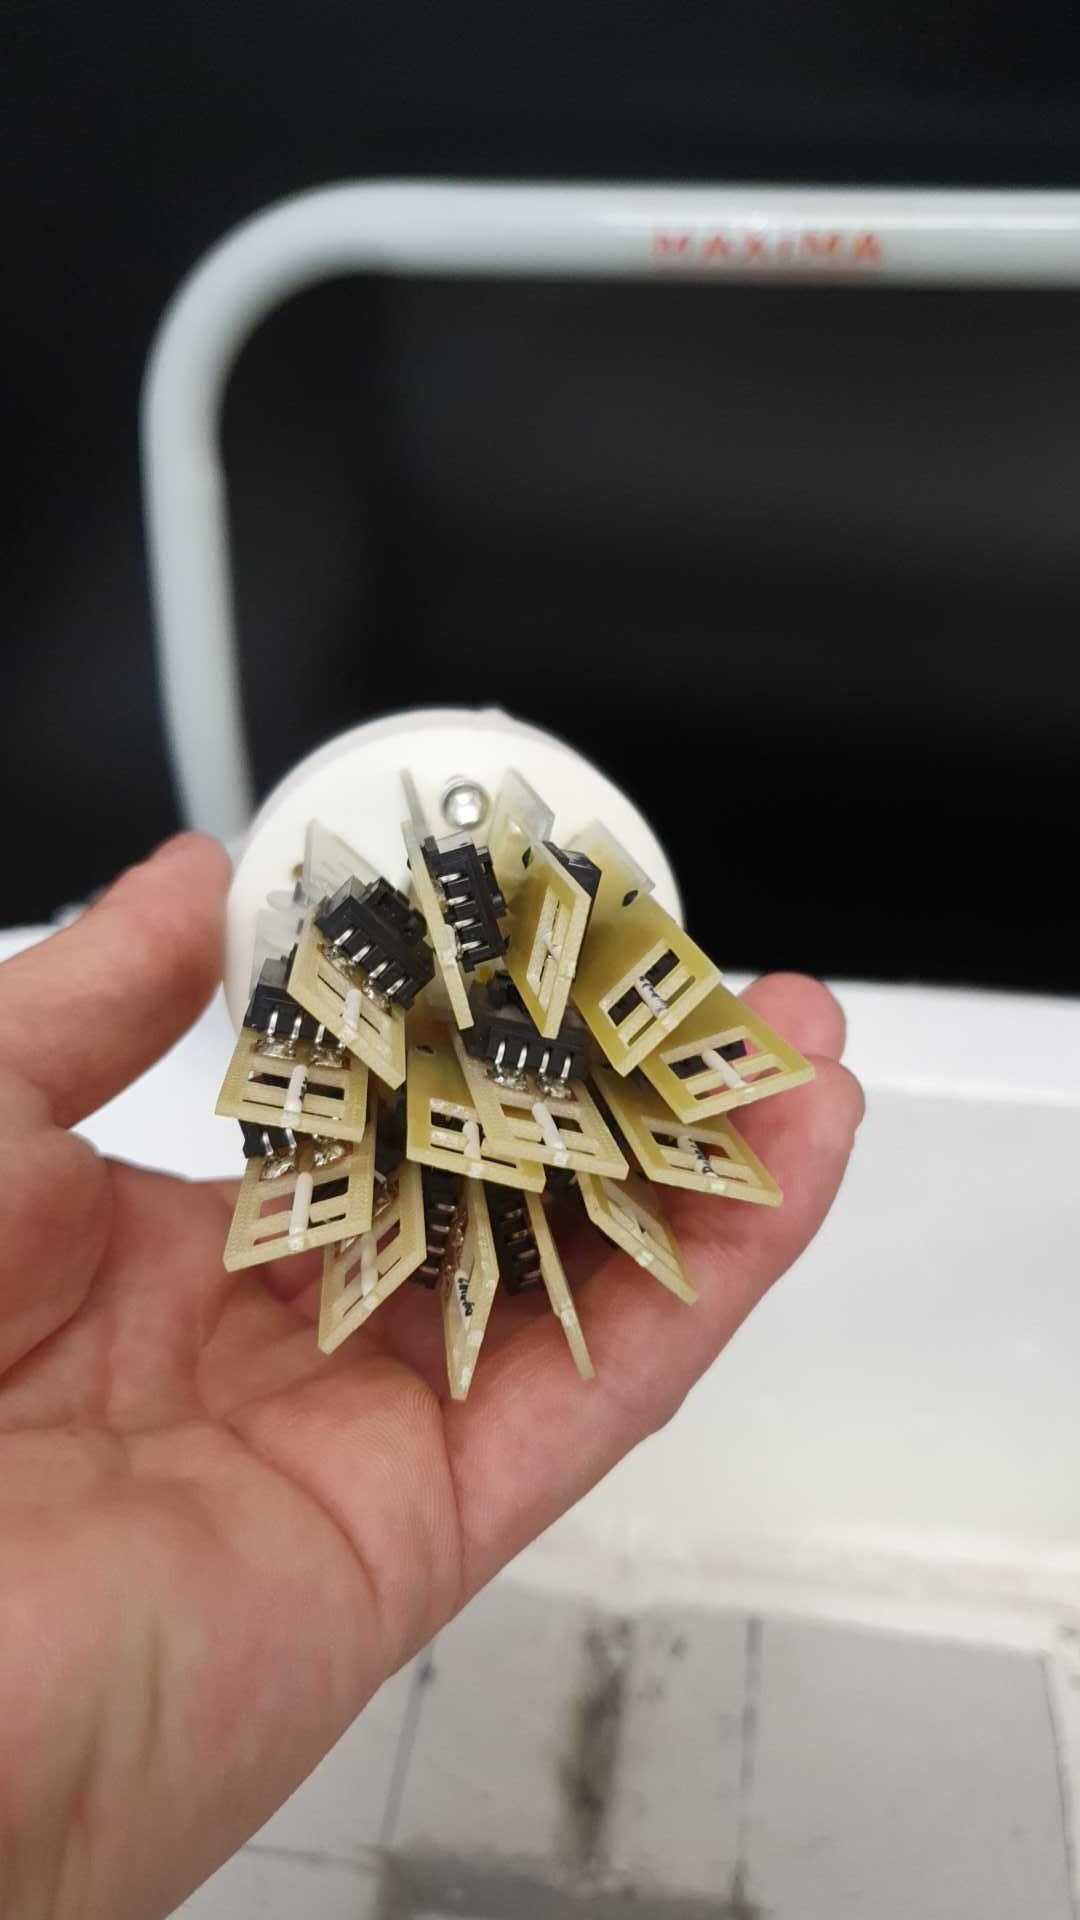
\includegraphics[width=0.3\textwidth, trim=0cm 4cm 0cm 7cm, clip]{images/figure_16_c.jpg}}
{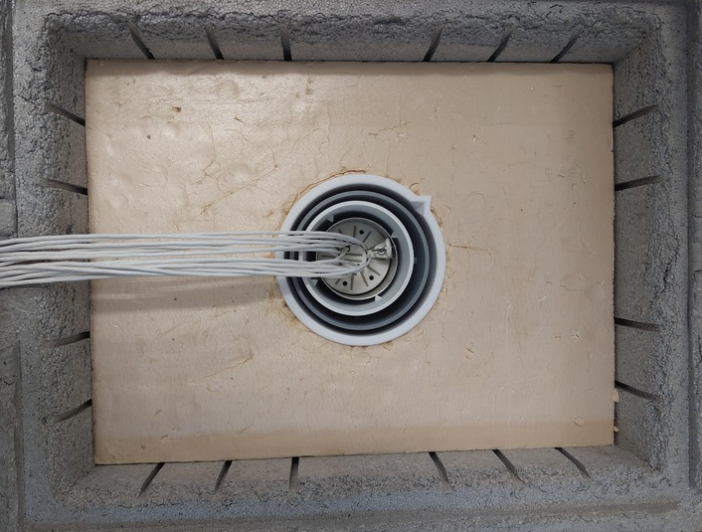
\includegraphics[angle=90,width=0.3\textwidth]{images/image.png}}
{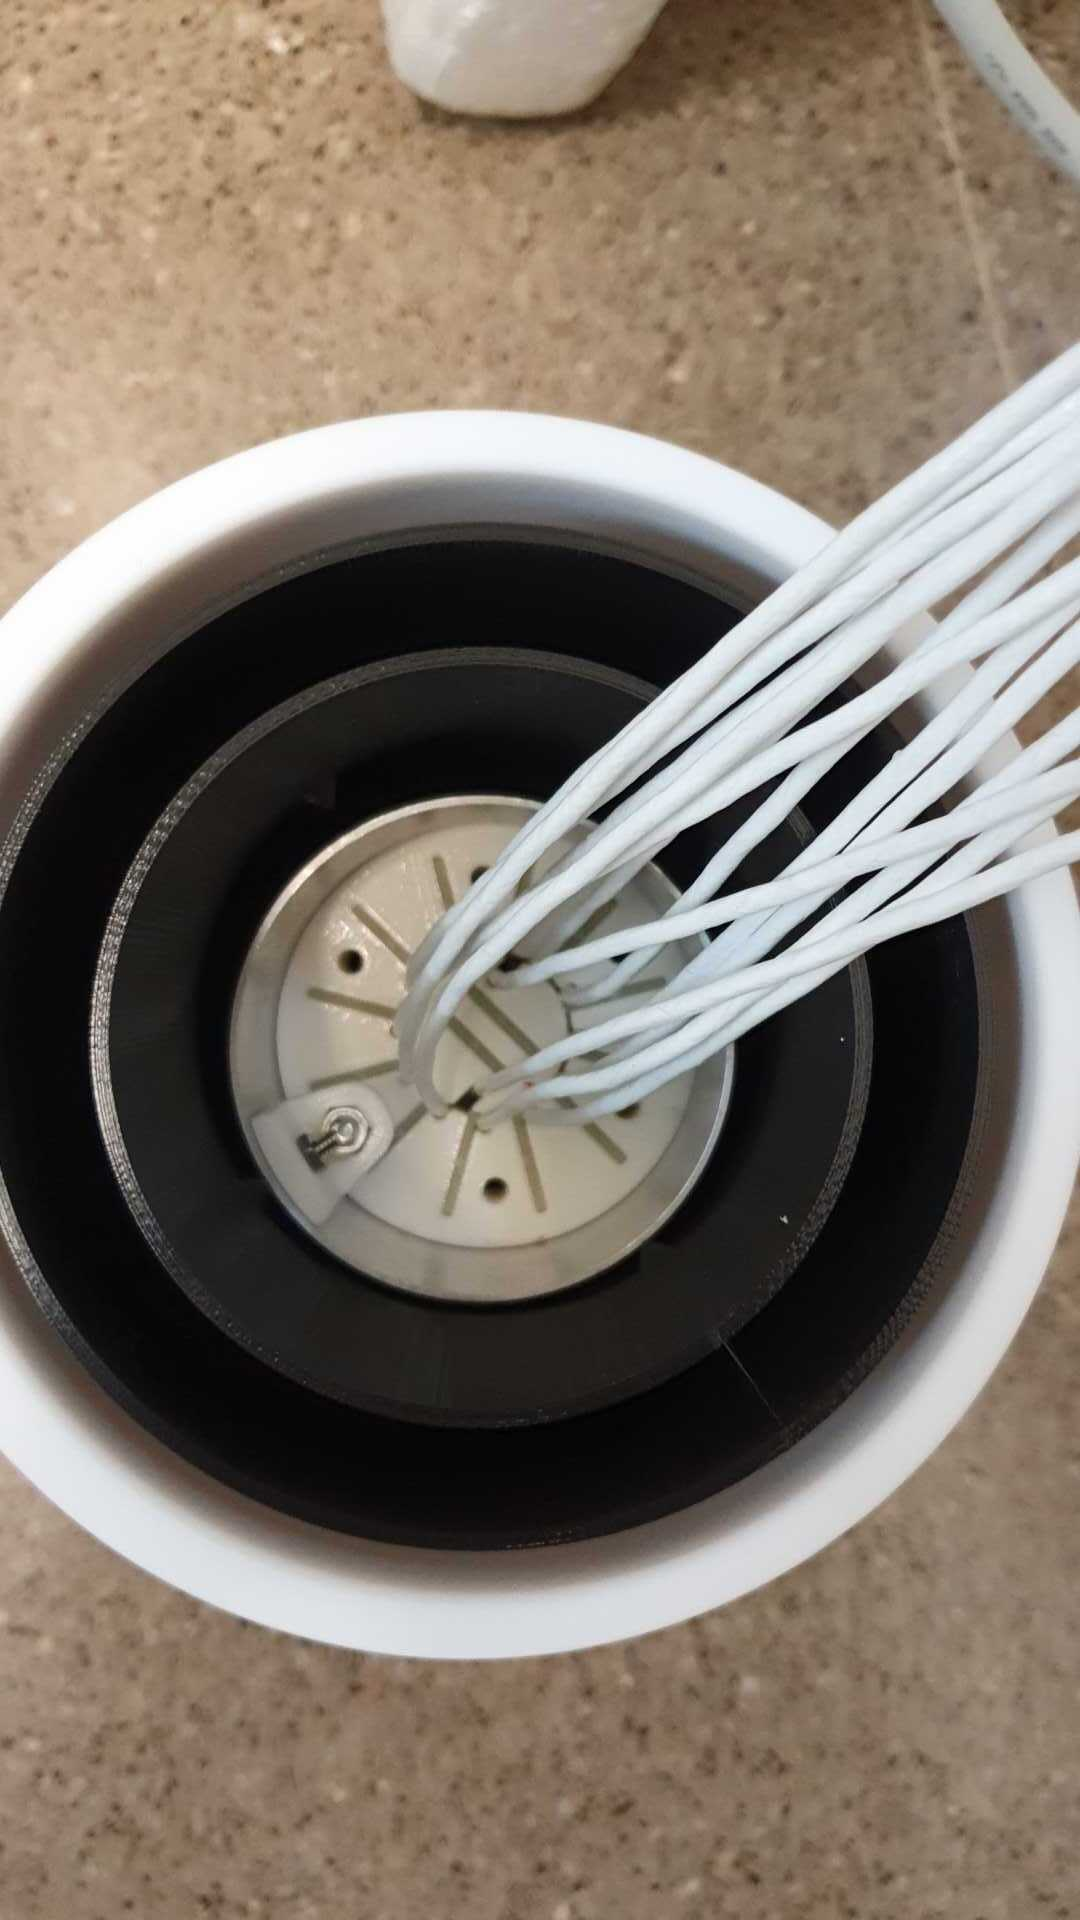
\includegraphics[width=0.303\textwidth,trim=0cm 6cm 0cm 7.45cm, clip]{images/figure_16_a.jpg}}
{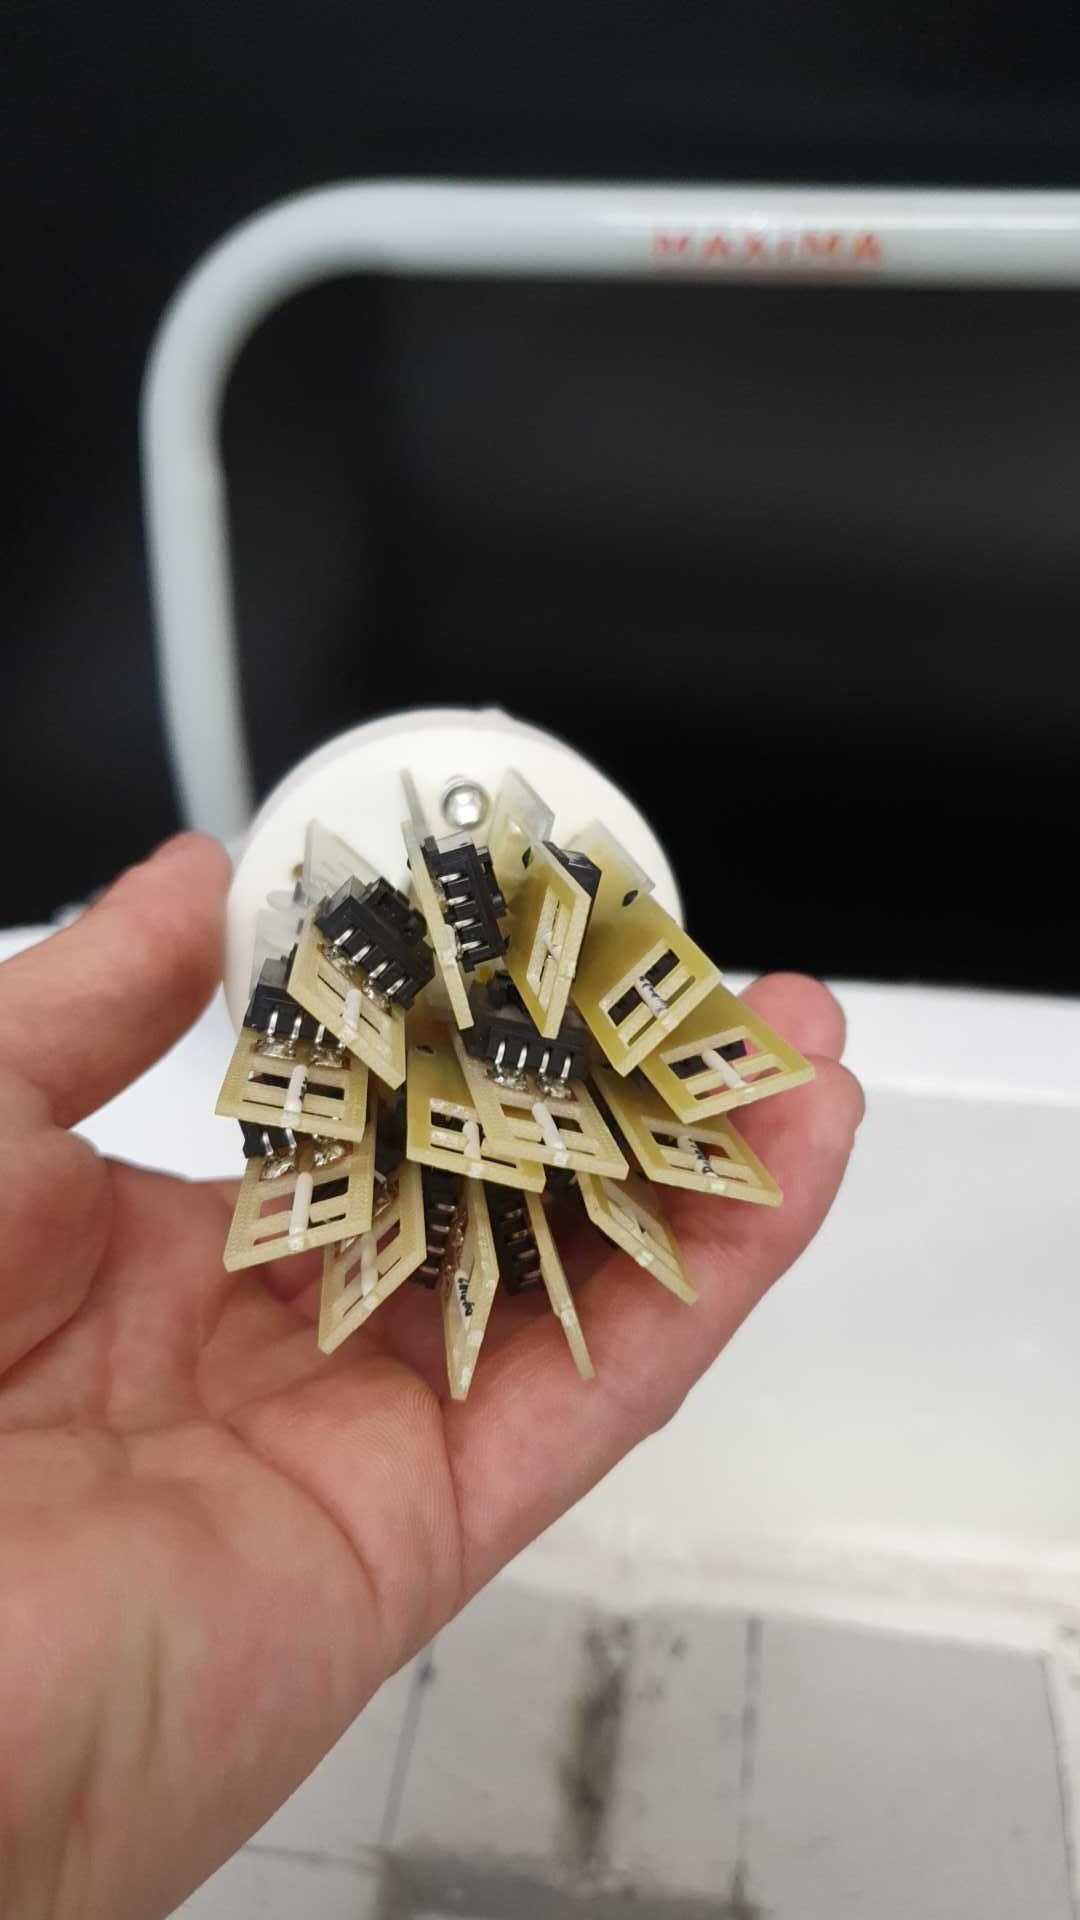
\includegraphics[width=0.3\textwidth, trim=0cm 7cm 0cm 10.4cm, clip]{images/figure_16_c.jpg}}
\caption{Left: The polystyrene box that hosts the calibration setup. Center: The four concentric volumes of the calibration setup. Right: The 12 corona sensors plus the 2 references.}
\label{fig:newSetup}
\end{figure}

%---------------------------------------------------
\subsection{Calibration procedure}
\label{sec:new_calib_procedure}

\noindent The sensor support was originally designed to accommodate two reference sensors in the center (see Fig. \ref{fig:newSetup}), enabling both the reference and tree calibration methods. However, it was soon observed that temperature variations between corona and reference sensors were significantly larger than those between any two corona sensors. This effect is attributed to the convection pattern inside the capsule, which is expected to have rotational invariance, and hence favour sensors disposed following a cylindrical symmetry. This can be observed in Fig. \ref{fig:refMethodDumpingJustification}-left, where the offset between two corona sensors is nearly constant in time in four independent measurements, and in Fig. \ref{fig:refMethodDumpingJustification}-right, where the offset between a corona and a reference sensor shows a more chaotic behaviour. Consequently, only the `tree' calibration method was considered during the calibrations after ProtoDUNE-SP decommissioning.

\begin{figure}[htbp]
\centering
{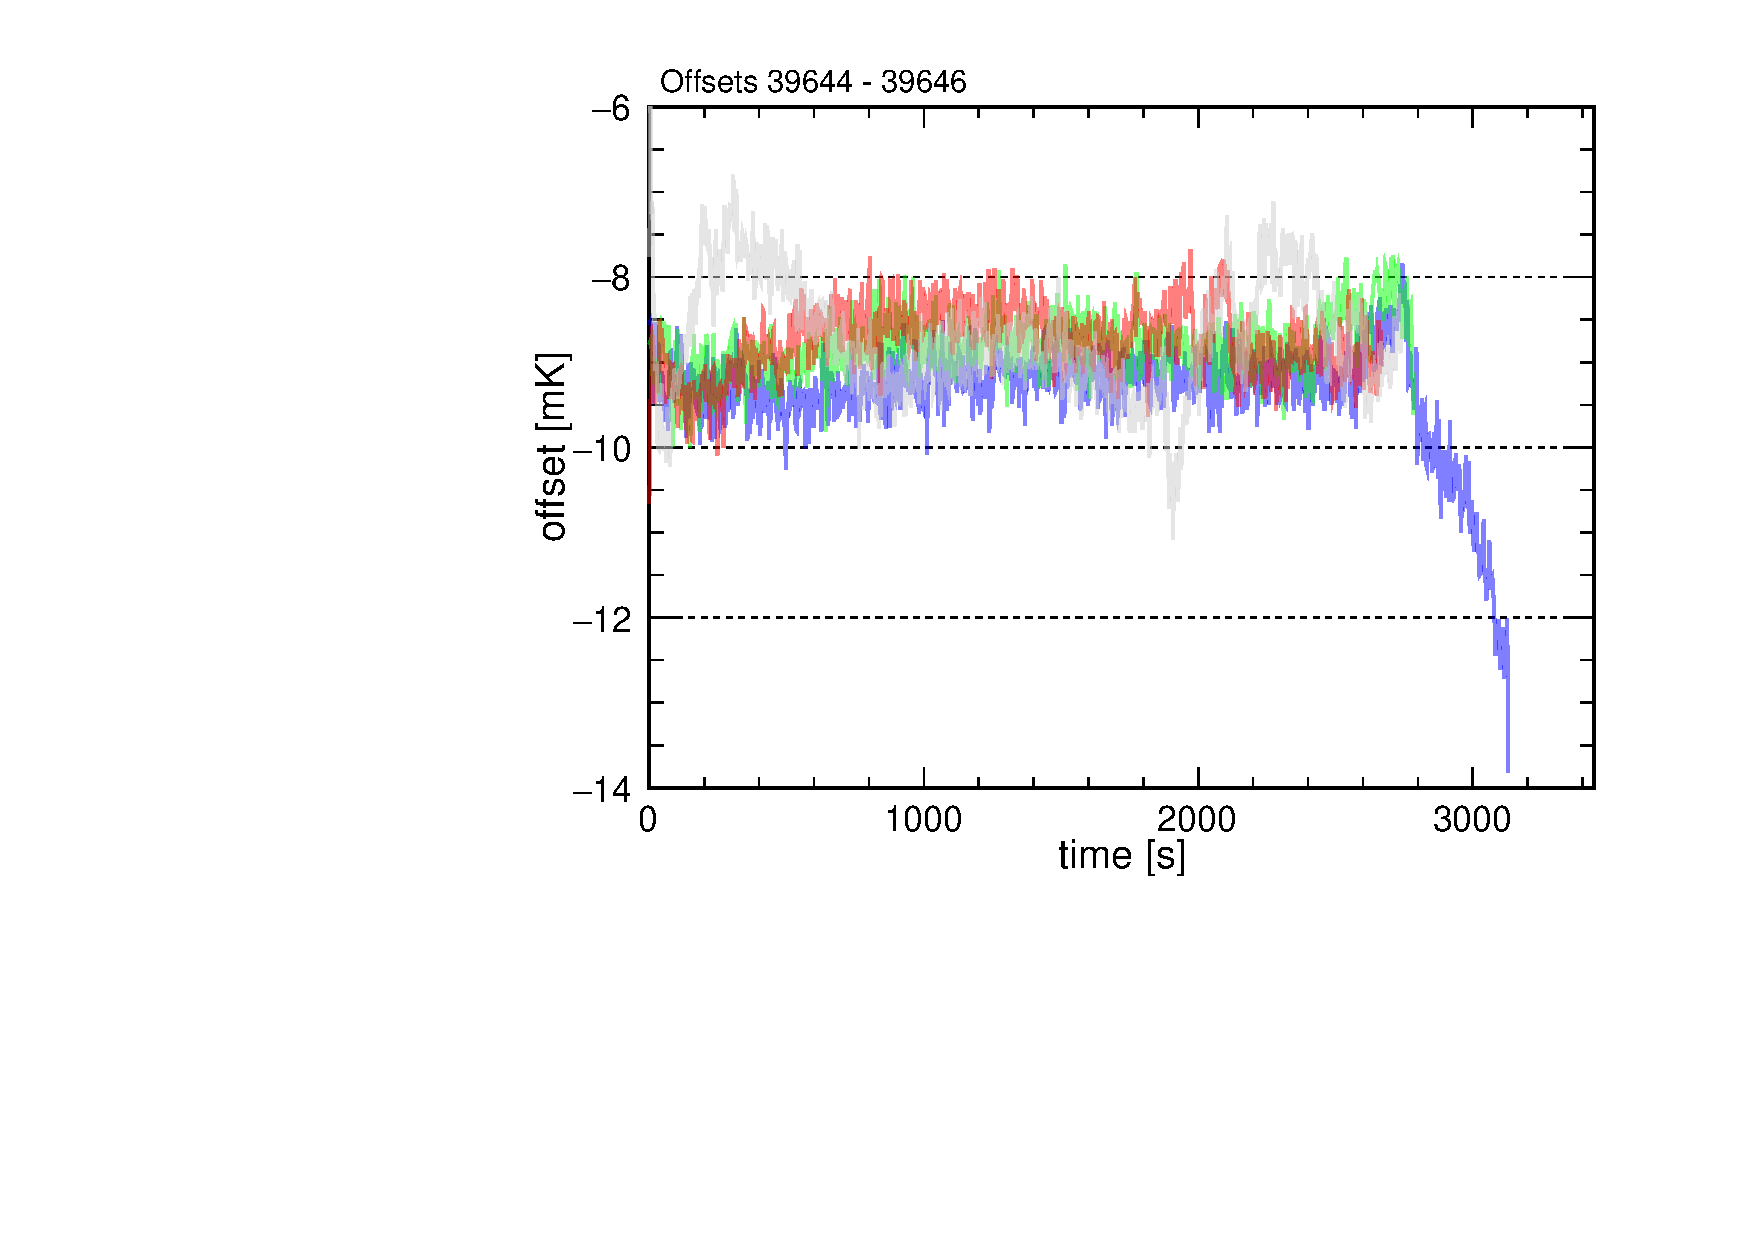
\includegraphics[width=0.45\textwidth]{images/figure_17_a.pdf}}
{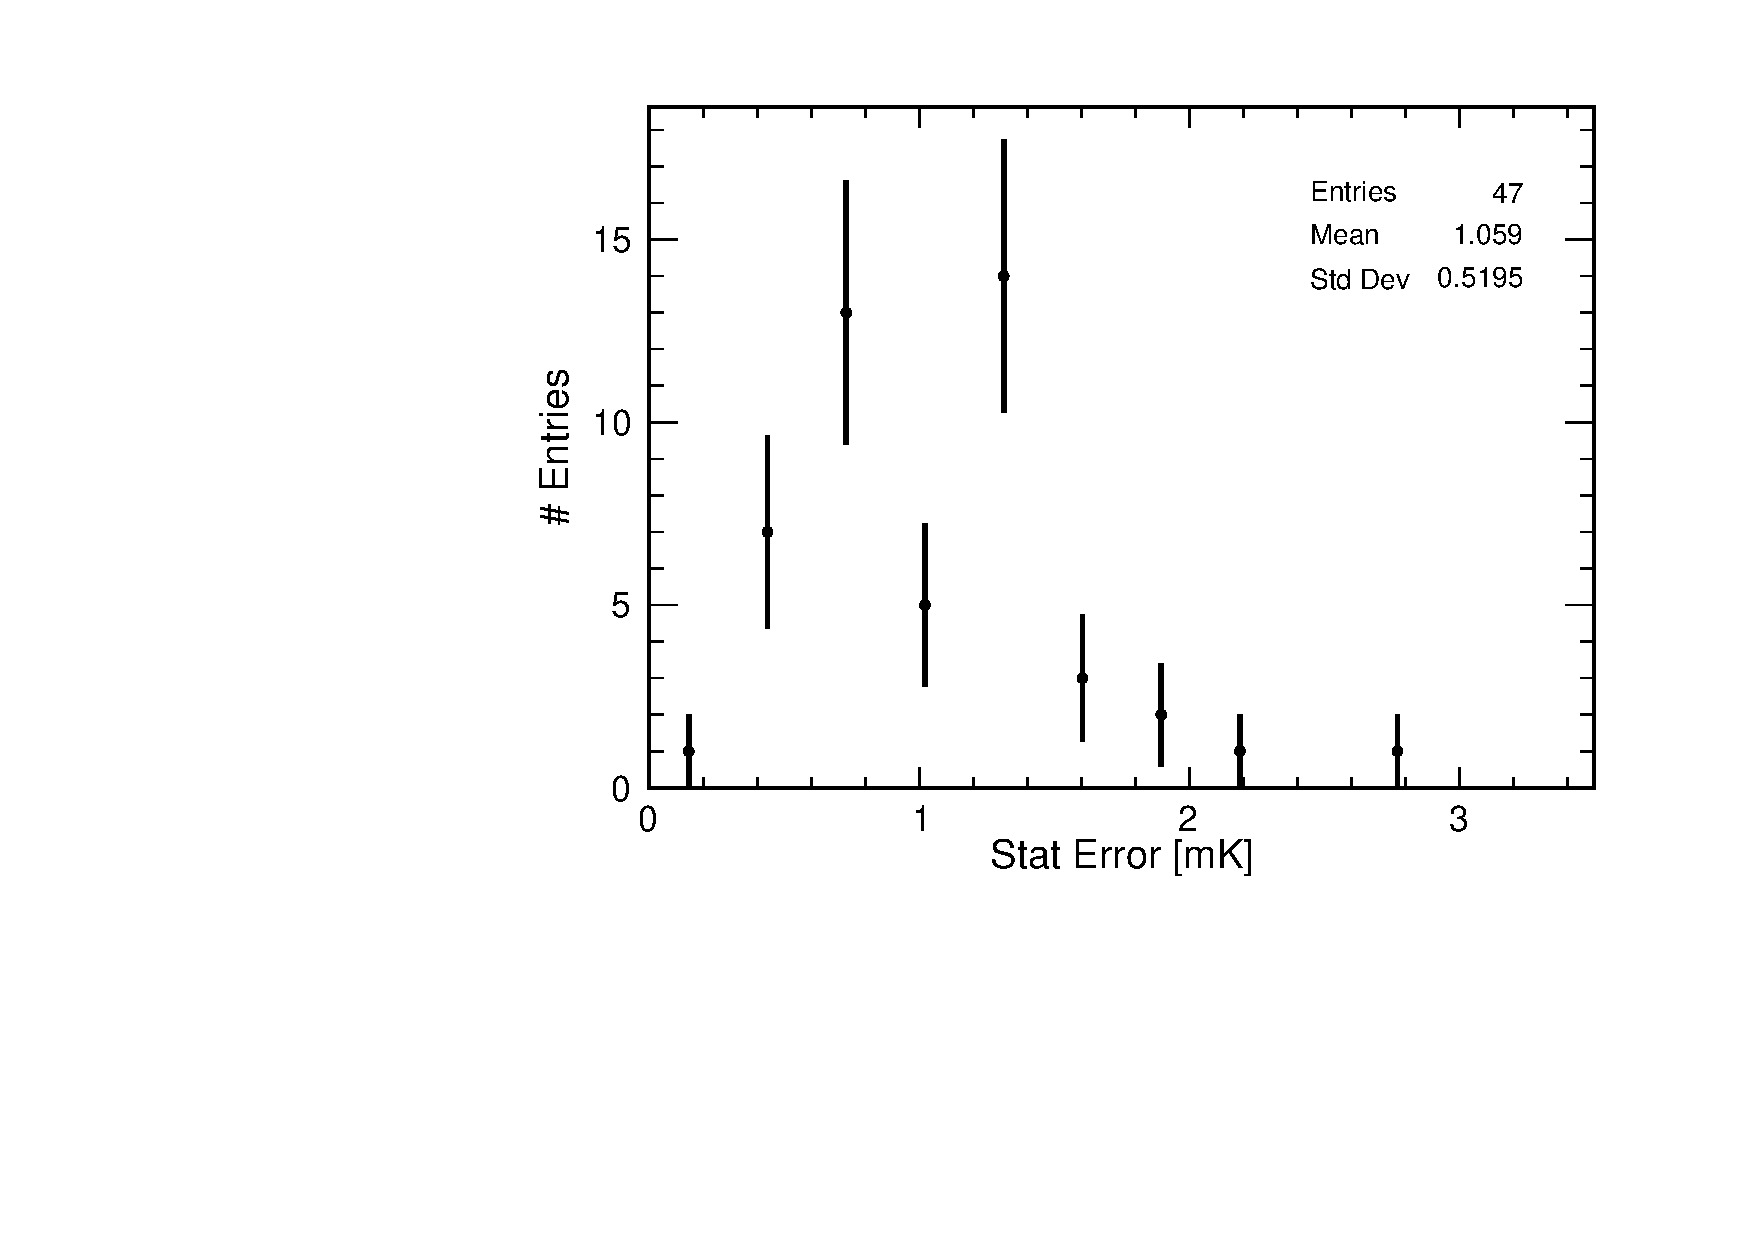
\includegraphics[width=0.45\textwidth]{images/figure_17_b.pdf}}
\caption{Left: The 4 measured offsets between two arbitrary sensors in the corona. Right: The 4 measured offsets between a sensor in the corona and one of the references, at the center.}
\label{fig:refMethodDumpingJustification}
\end{figure}

The new calibration tree, shown in Fig. \ref{fig:newCalibrationStrategy}, contemplates four 12-sensors sets in the first round, and a unique second round with three promoted sensors from each of the sets in the first round. With this scheme, promoted sensors only suffer 8 baths, avoiding the necessity of a time-walk correction.

\label{sec:newCalibrationStrategy}
\begin{figure}[htbp]
\centering
{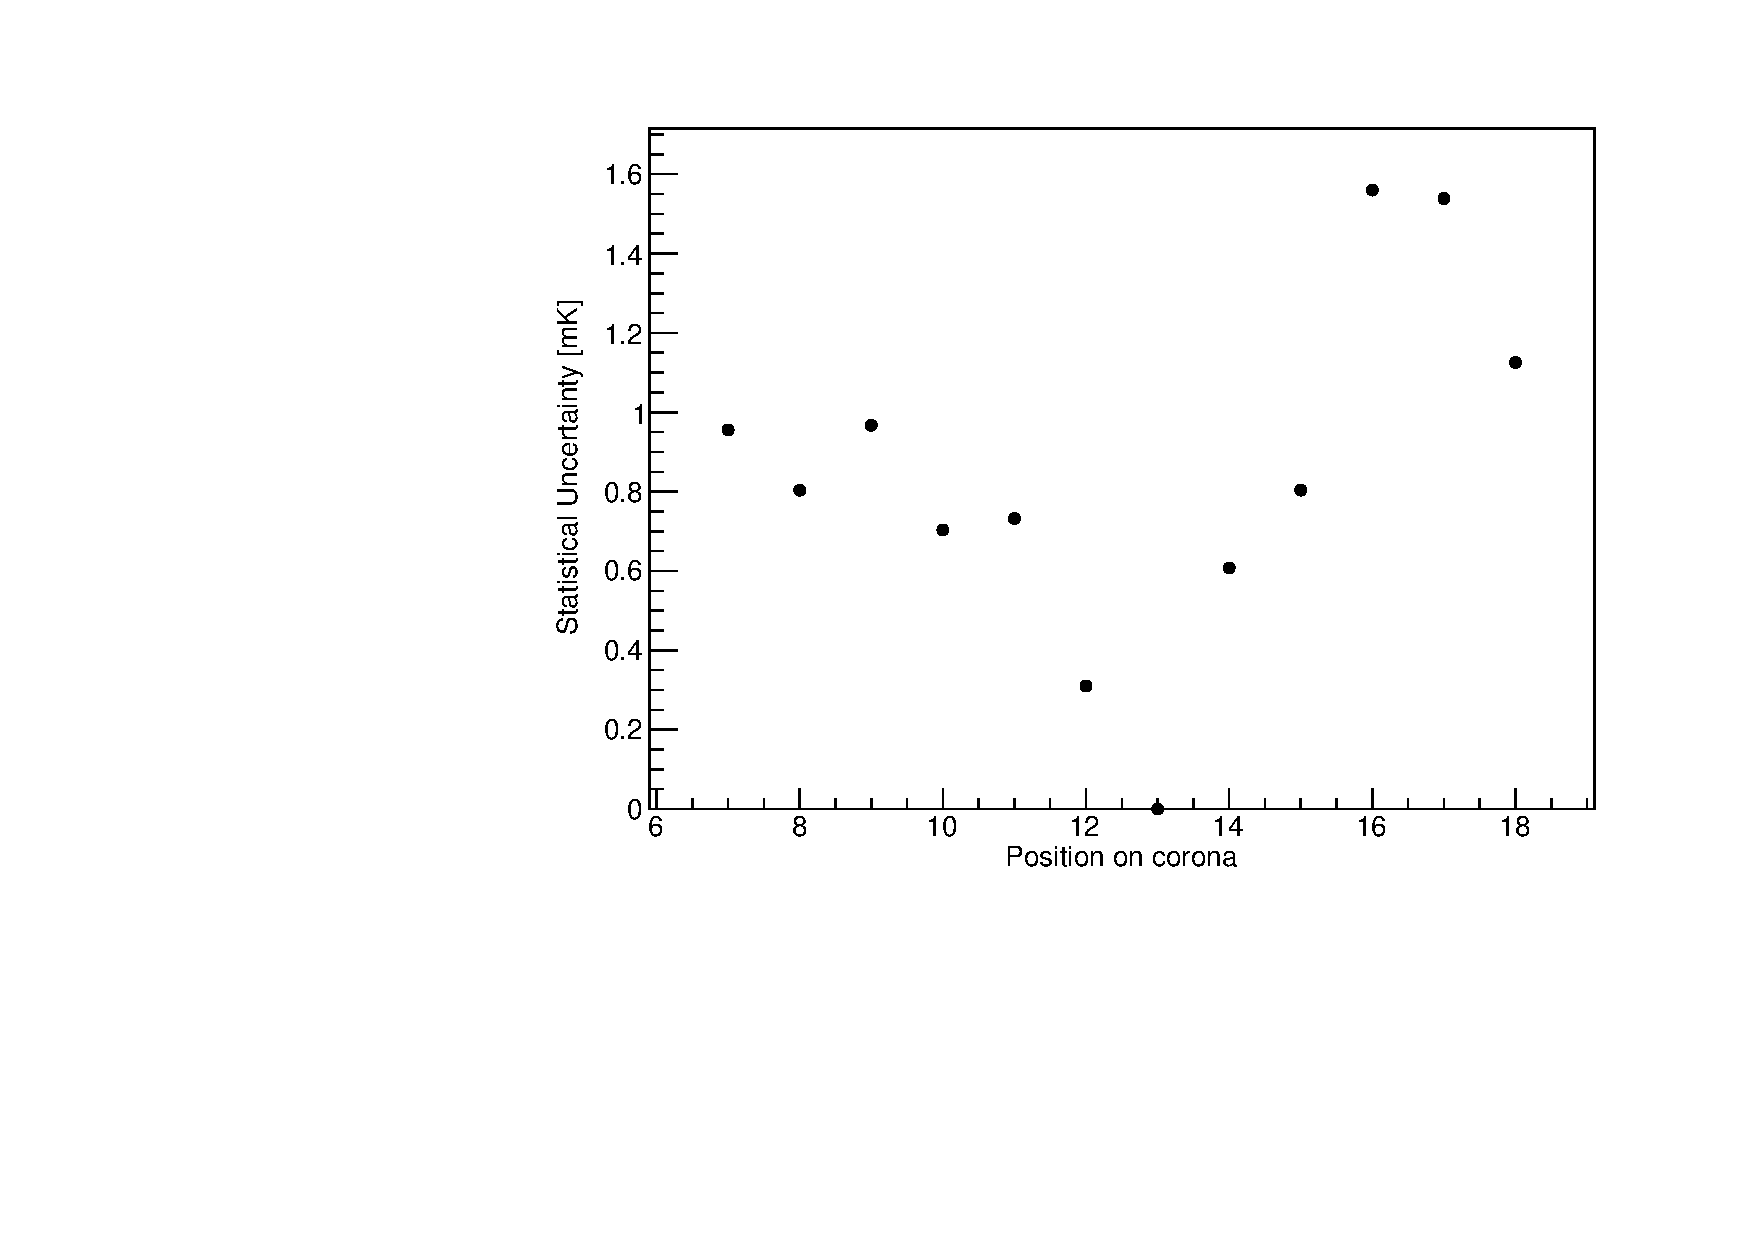
\includegraphics[width=0.9\textwidth]{images/figure_18.pdf}}
\caption{Schematic of the calibration sequence used with the new setup. Each of the sets contains 12 sensors, all of them placed in the corona, plus 2 references at the center. Sensors in bold in the first round are promoted to the second round.}
\label{fig:newCalibrationStrategy}
\end{figure}

The experimental procedure is similar to the one presented in Sec.~\ref{sec:old_calib}. Two small variations were introduced. First, the several concentric containers are cooled down for 40 minutes before introducing the aluminium capsule for the first time in a day, slightly improving the results of the first calibration run. Second, the warm up process is accelerated using a heat gun, avoiding the use of water.

%----------------------------------------------------------
\subsection{Calibration results}
\label{sec:new_calib_results}

\noindent A sensor from the second round is chosen as the reference, as this minimizes the number of operations required for the non-promoted sensors. Since each set includes three promoted sensors, there are three \textcolor{red}{linearly independent} ways to compute the offset relative to the reference for the nine non-promoted sensors in that set. The calibration constant for these sensors is calculated as the weighted average of the three “paths”, with its uncertainty given by the standard deviation of these three values. The offset uncertainty used in the weighted average for each of the three paths is computed by quadratically summing the individual uncertainties (as in Fig.~\ref{fig:newCalib_stat}) of all terms contributing to the offset along that specific path. Sensor 40525 is adopted as the reference for the remainder of the analysis.

Fig.~\ref{fig:newCalib_stat} shows the distribution of the repeatability (defined in Sec.~\ref{sec:results_first_round}) for the three new calibrations mentioned in Table~\ref{tab:calib}. The values obtained are slighly worst than in the 2018 calibration campaign, which is somehow expected given the increased capsule size and the larger distance between sensors. This hypothesis is supported by Fig.~\ref{fig:newCalib_statVsChannel}, showing the repeatability as a function of the distance to the reference sensor in the corona for a particular measurement. However, there is no substantial difference between the repeatability obtained for LN2 and LAr calibrations.

% Using the same logic presented in Sec.~\ref{sec:calib_procedure}, the offset between any pair of sensors can be computed by following a certain path in the tree. To minimise the statistical error, all offsets are referenced to a sensor in the second round, 40525, chosen as reference. The previous reference, 39656, was discarded since it was damaged during ProtoDUNE-SP decommissioning. Fig.~\ref{fig:newCalib_stat} shows the distribution of the repeatability (defined in Sec.~\ref{sec:results_first_round}) for the three new calibrations mentioned in Table~\ref{tab:calib}. In all three cases the error is slightly above 1 mK. As expected, this error is larger than in the 2018 calibration mainly due to the increased size of the inner volume and the larger distance between sensors. This hypothesis is supported by Fig.~\ref{fig:newCalib_statVsChannel}, showing the statistical error as a function of the distance to the reference sensor in the corona for a particular measurement. However, there is no substantial difference between the repeatability obtained for LN2 and LAr calibrations.%, indicating that convection inside the capsule should be similar for both liquids.

% \begin{figure}[htbp]
% \centering
% {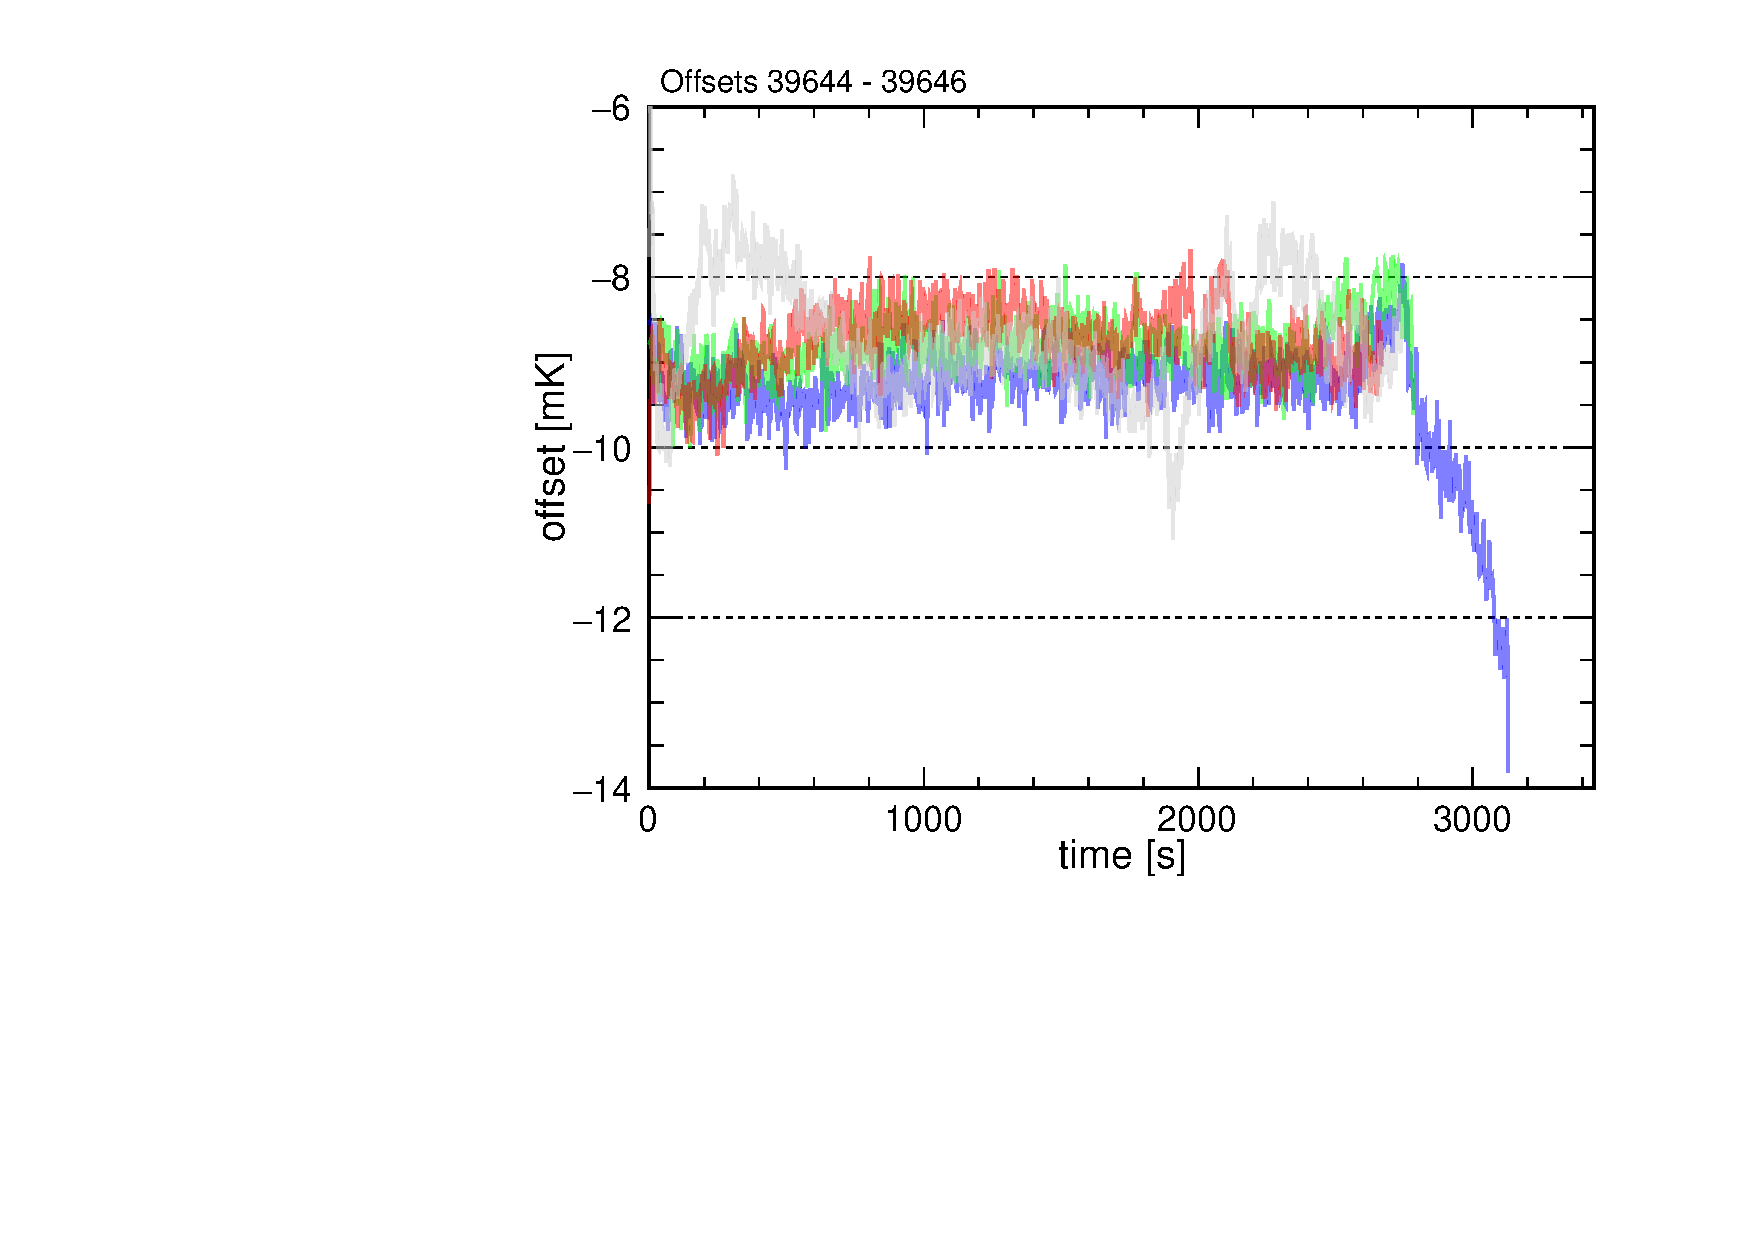
\includegraphics[width=0.33\textwidth]{images/figure_17_a.pdf}}{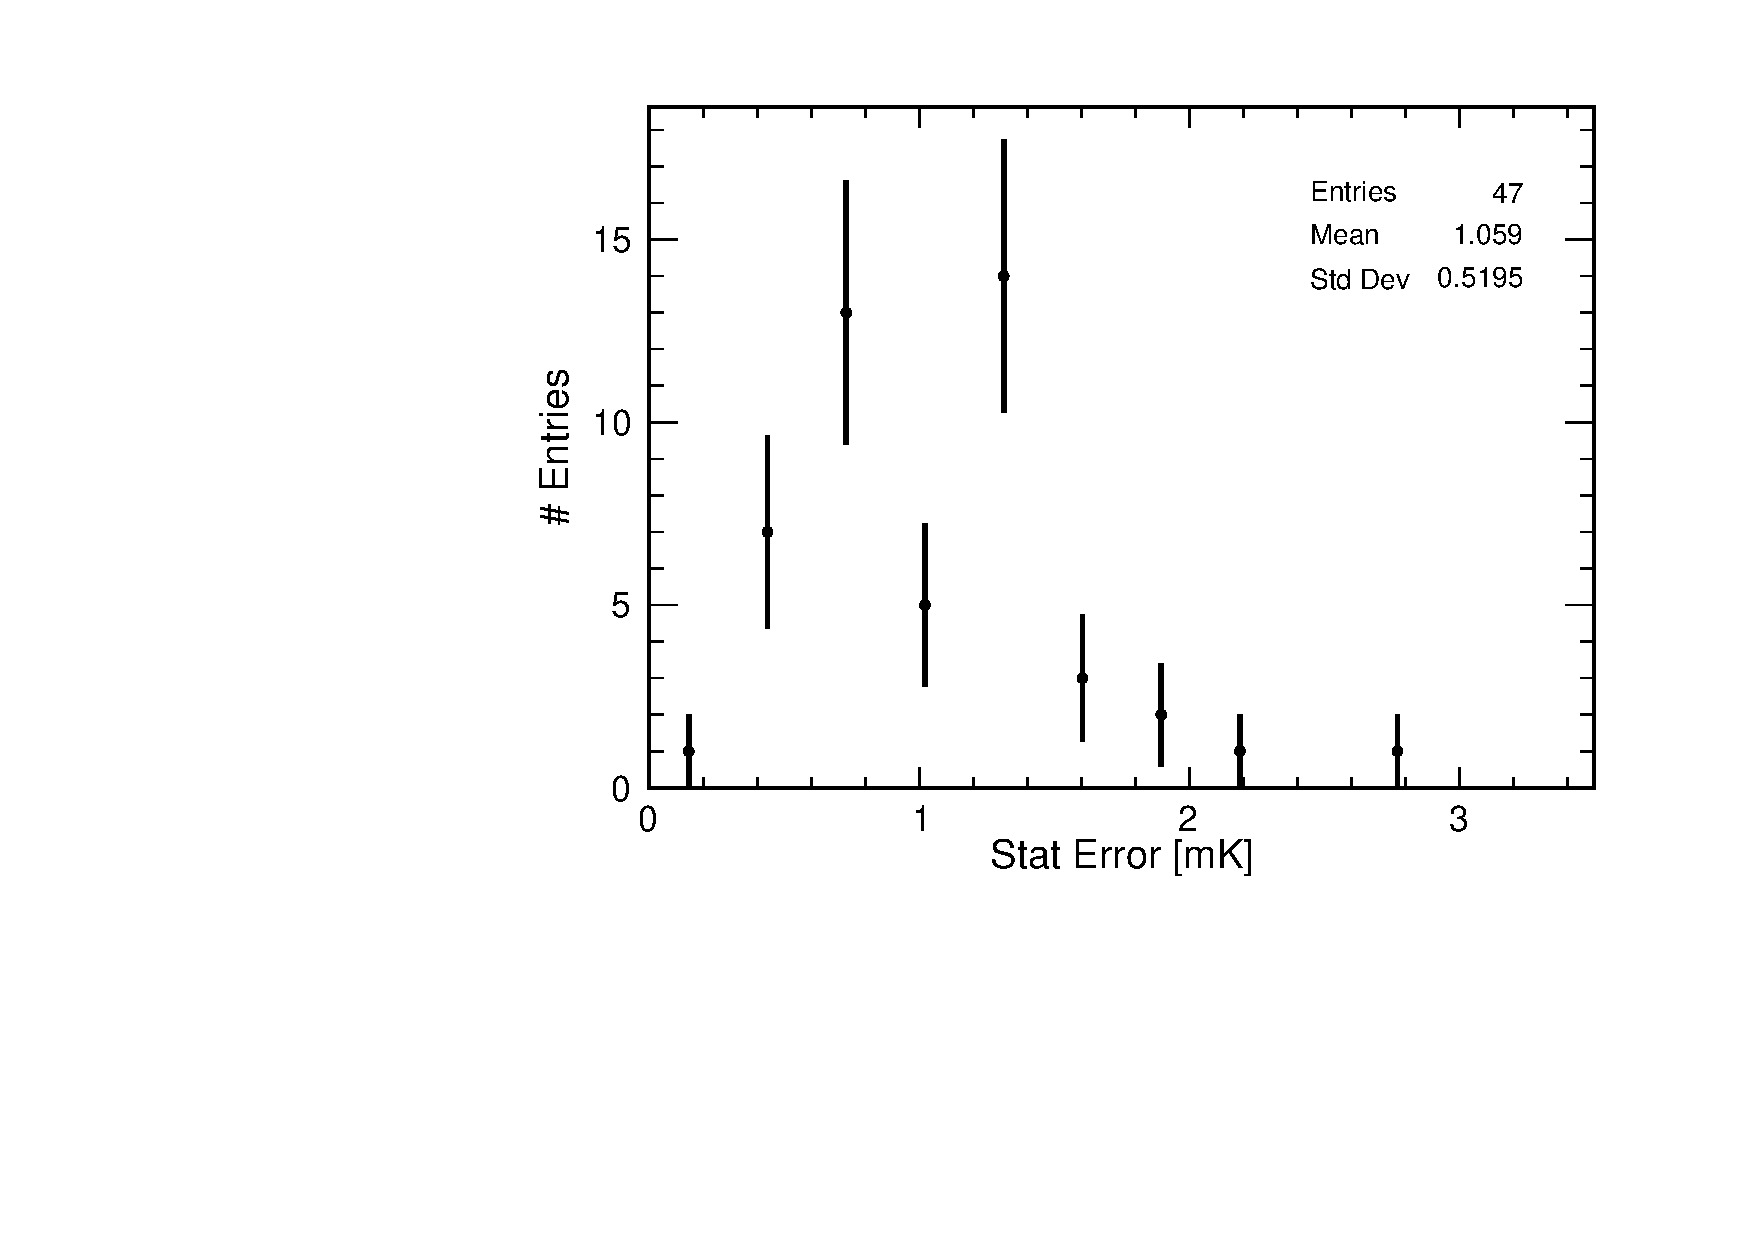
\includegraphics[width=0.33\textwidth]{images/figure_17_b.pdf}}{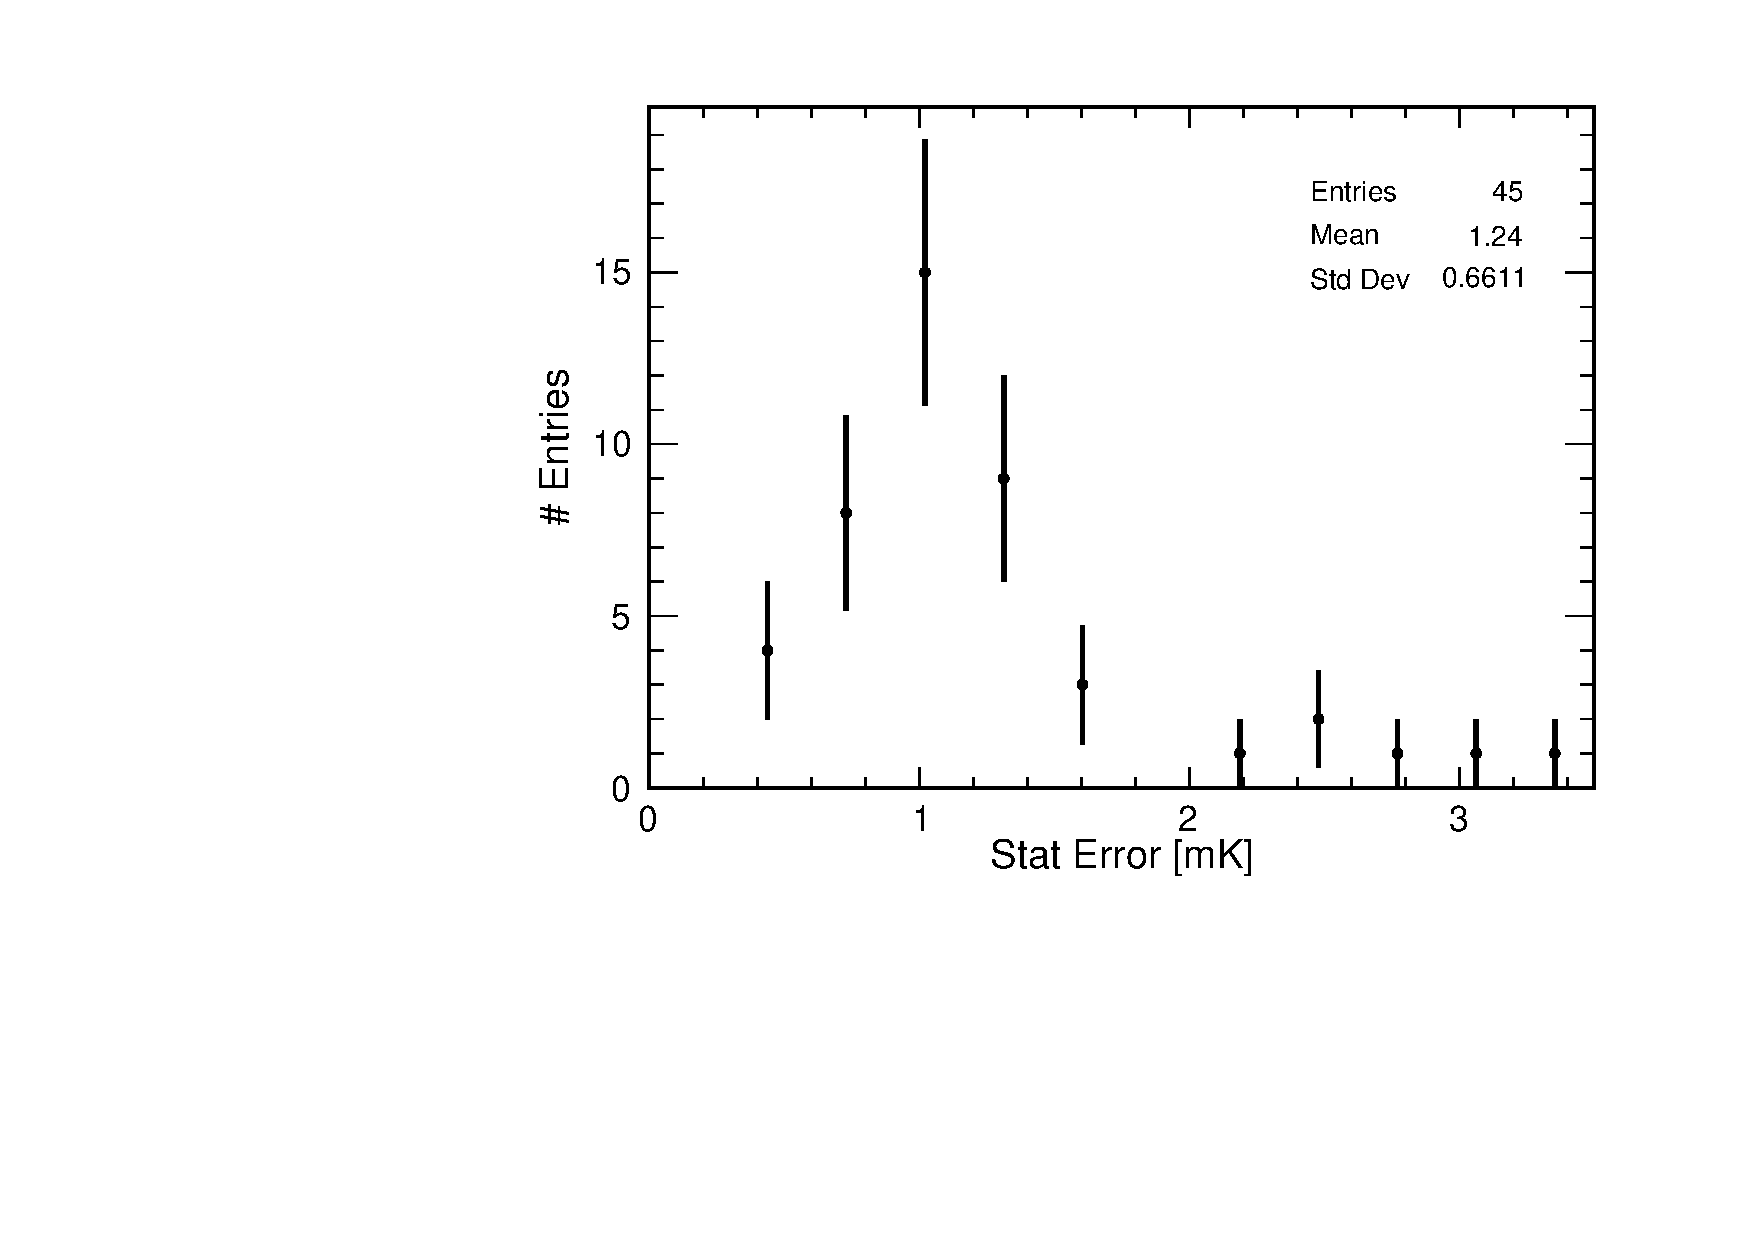
\includegraphics[width=0.33\textwidth]{images/figure_17_c.pdf}}
% \caption{Statistical error distribution for the new calibrations. Left: LN2-2022. Middle: LN2-2023, Right:LAr-2023}
% \label{fig:newCalib_stat}
% \end{figure}

\begin{figure}[htbp]
    \centering
    {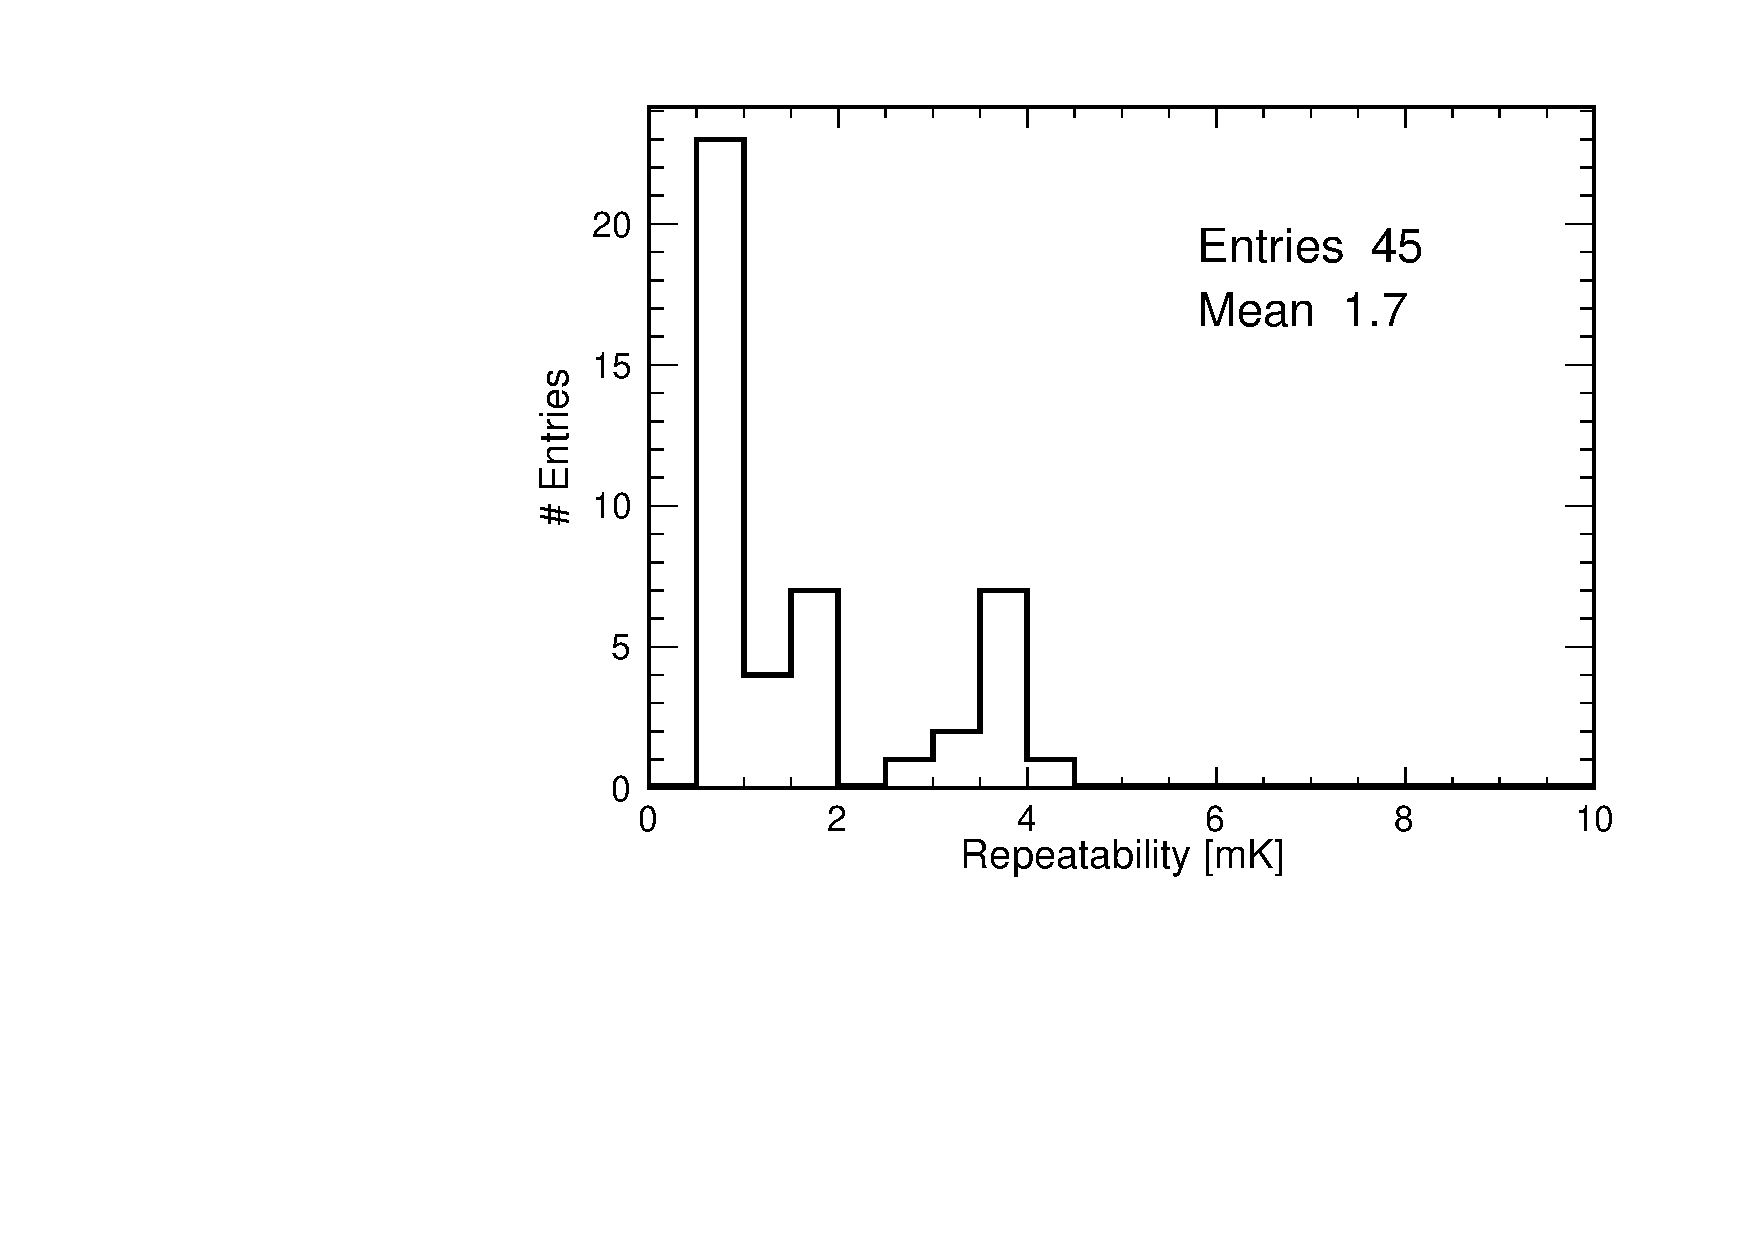
\includegraphics[width=0.33\textwidth]{images/figure_19_a.pdf}}{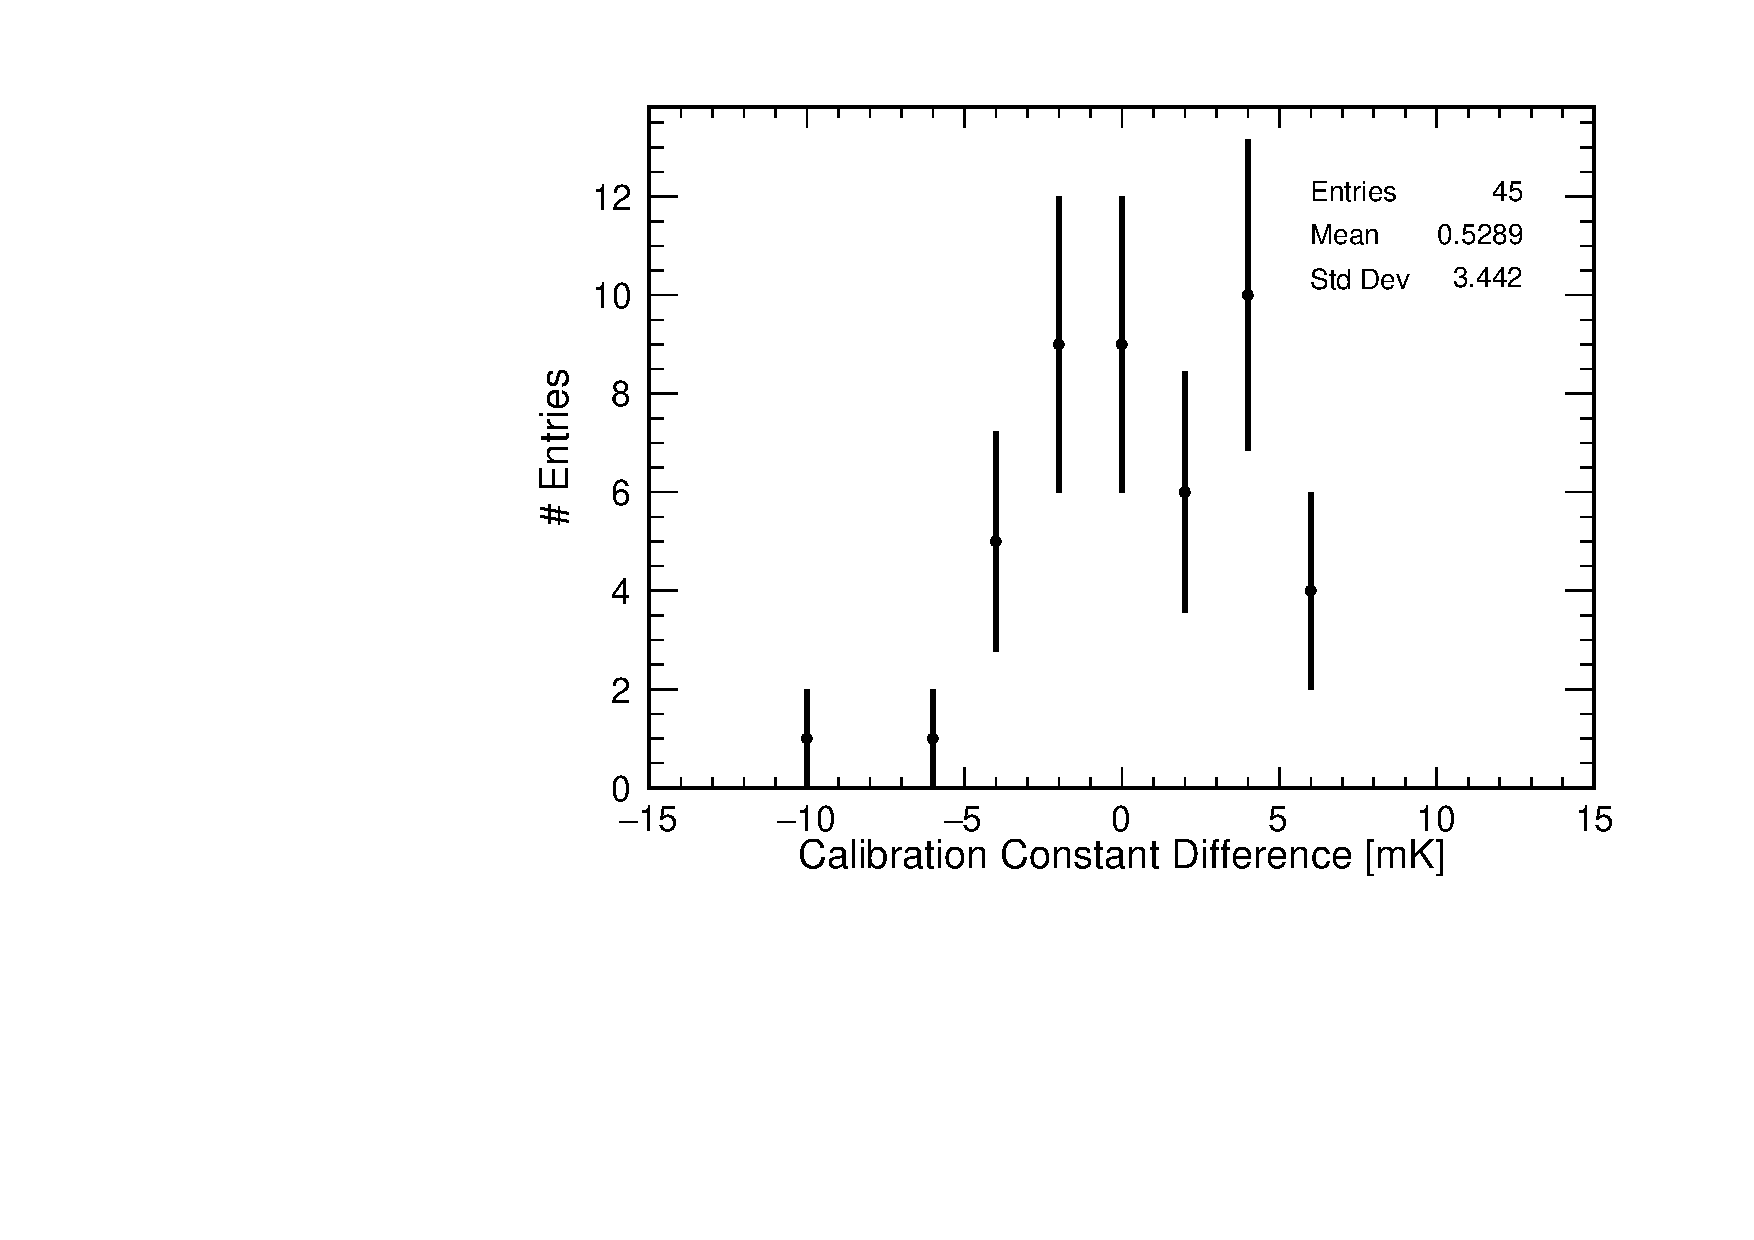
\includegraphics[width=0.33\textwidth]{images/figure_19_b.pdf}}{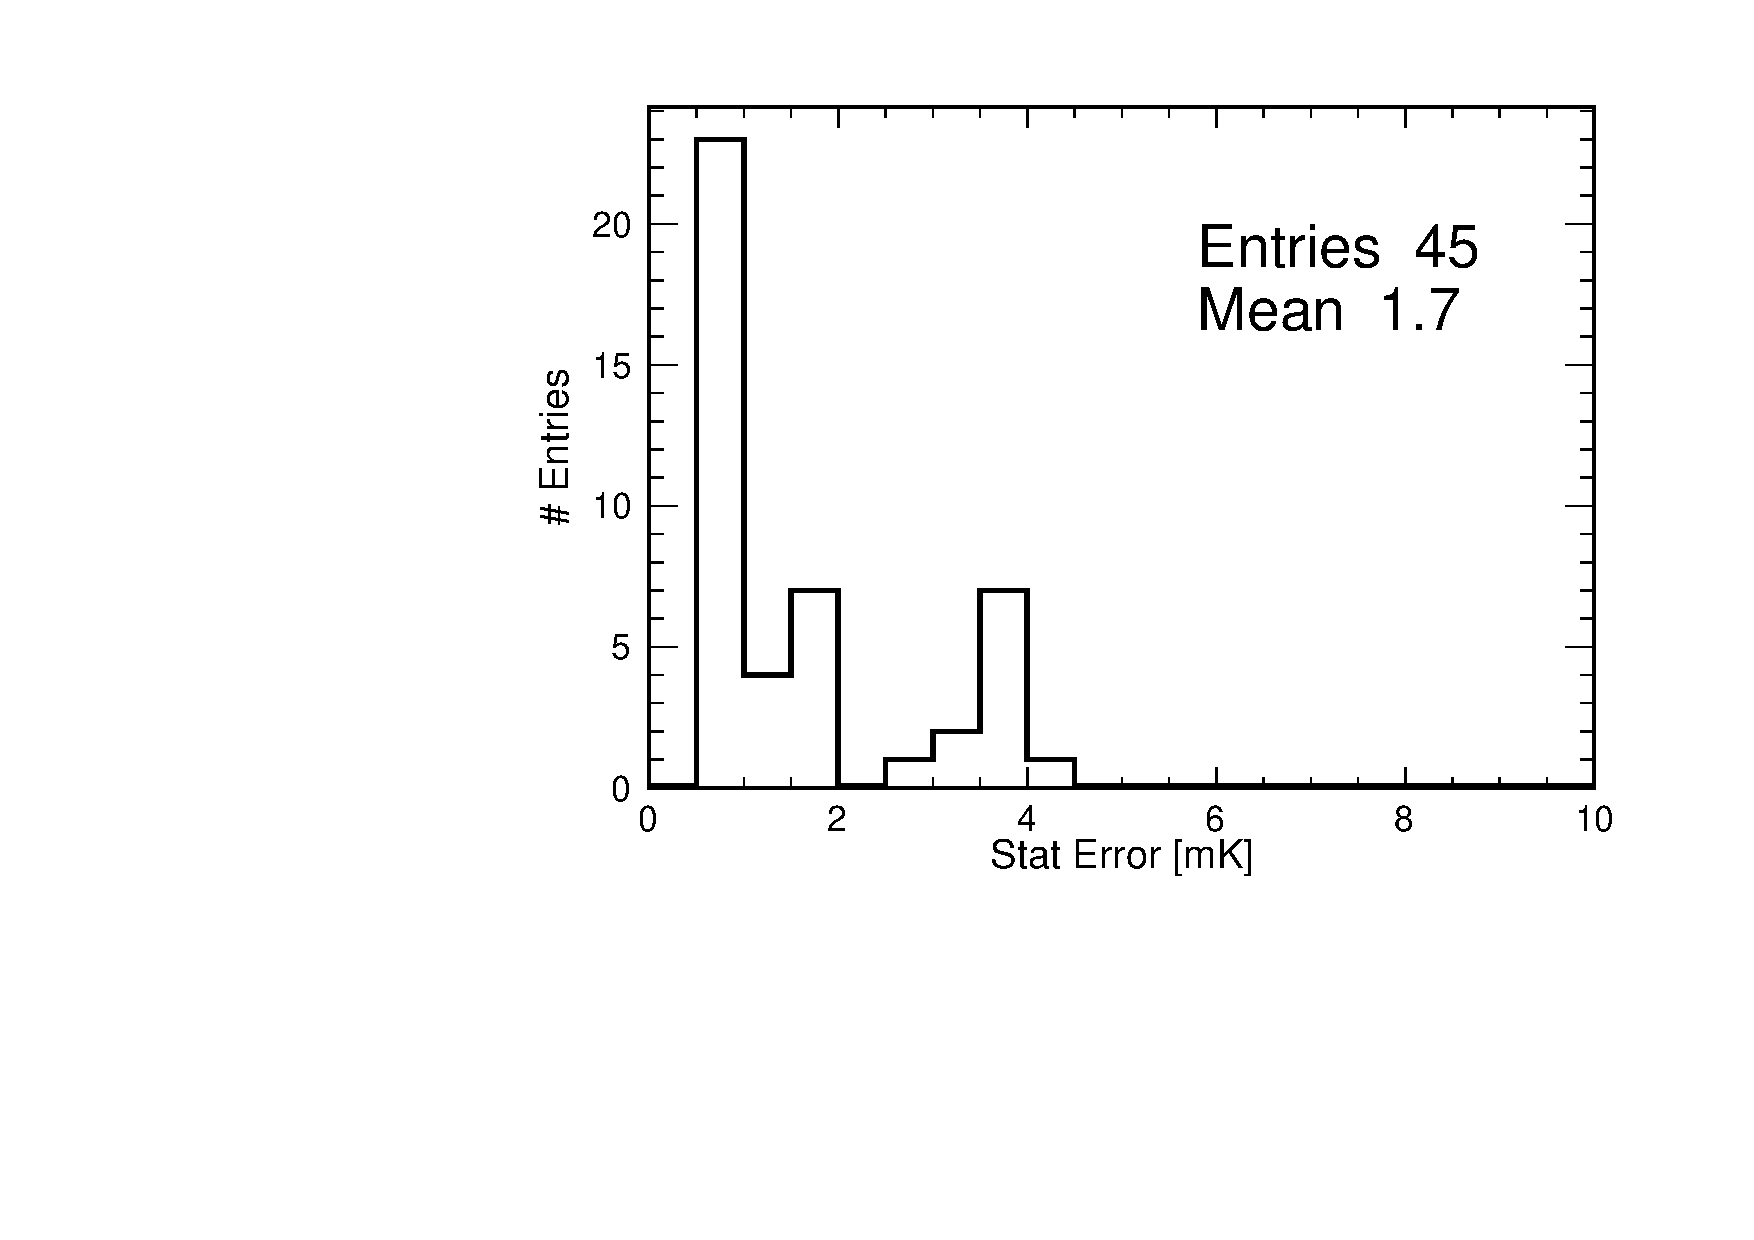
\includegraphics[width=0.33\textwidth]{images/figure_19_c.pdf}}
    \caption{Repeatability distribution for the new calibrations. Left: LN2-2022. Middle: LN2-2023. Right:LAr-2023. LAr-2023 includes two additional sensors, absent from earlier calibration campaigns, which were replaced after being damaged during the decommissioning of ProtoDUNE-SP.}
    \label{fig:newCalib_stat}
    \end{figure}

\begin{figure}[htbp]
\centering
{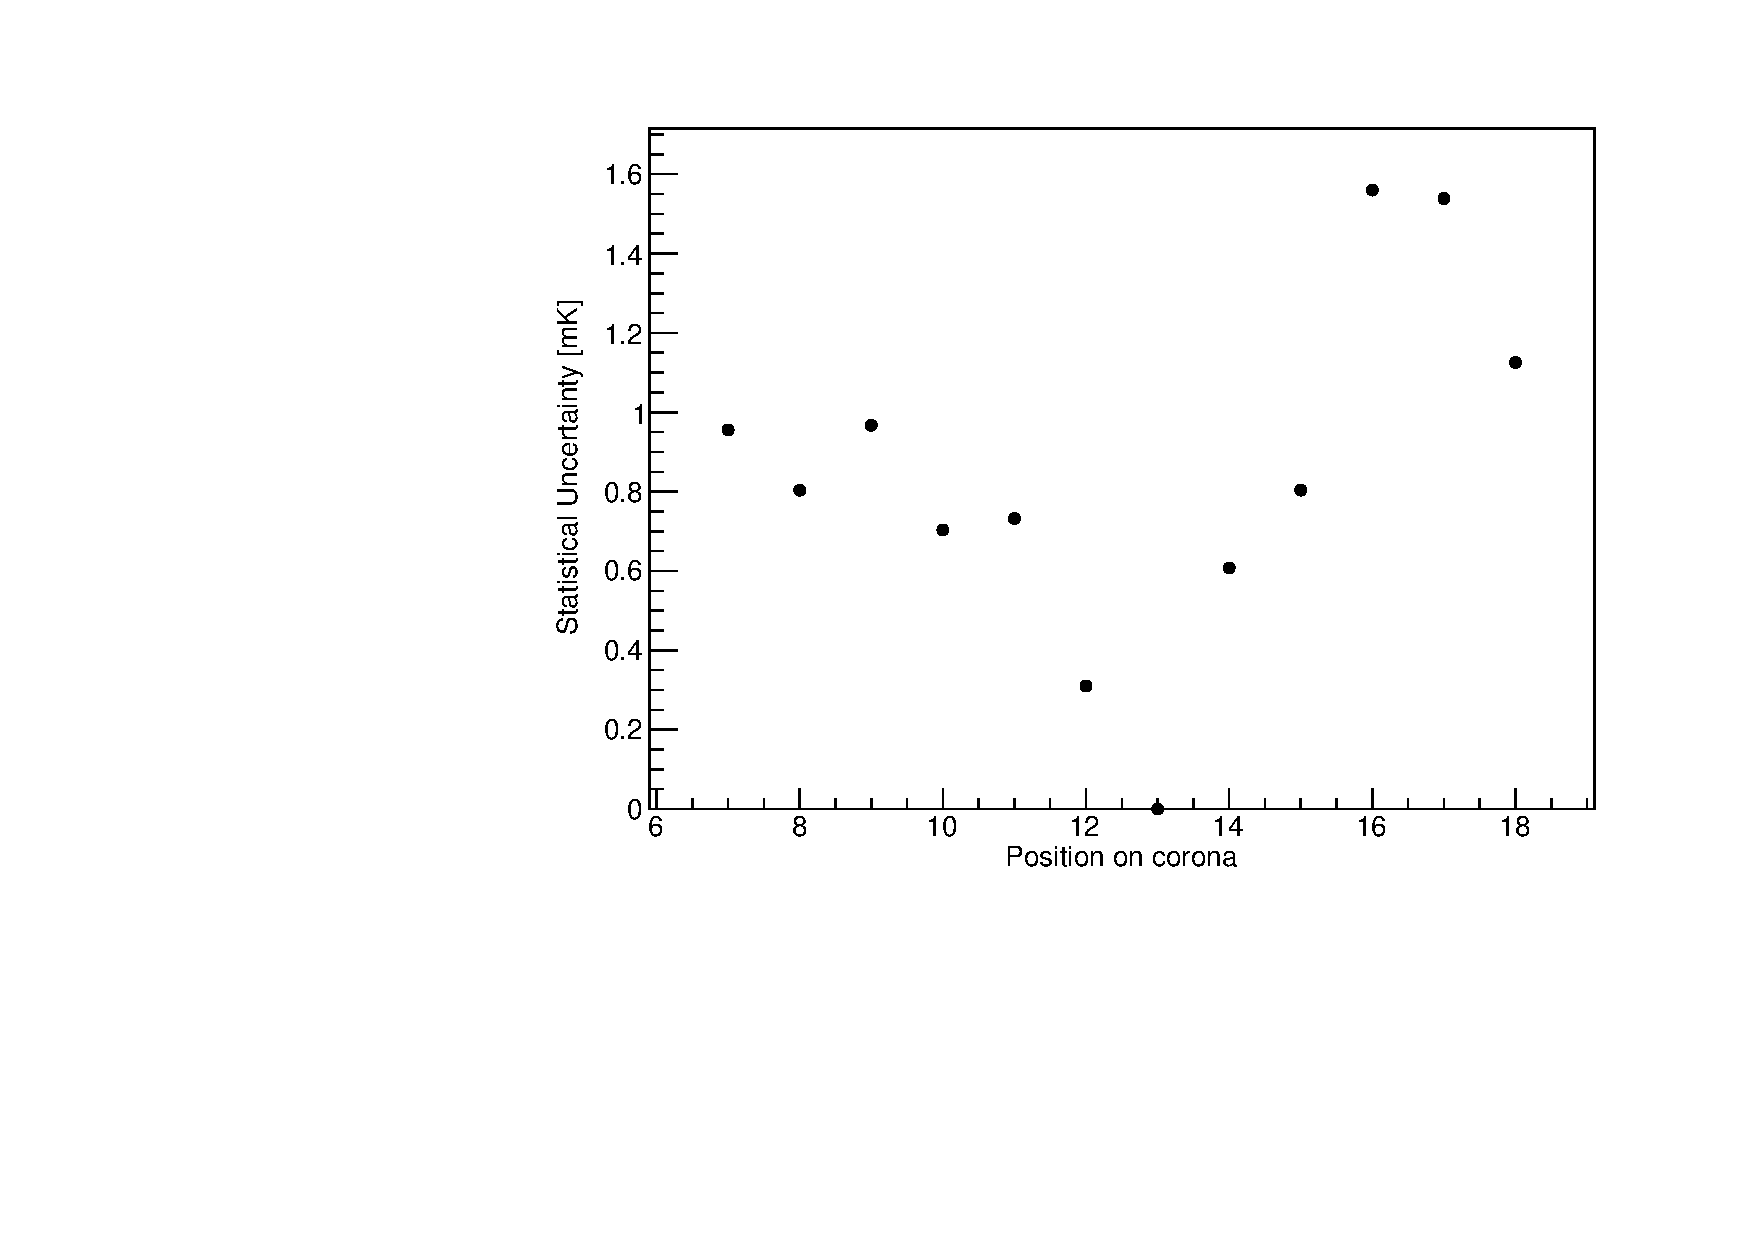
\includegraphics[width=0.65\textwidth]{images/figure_20.pdf}}
\caption{Repeatability as a function of position in the corona for the first set of the LAr-2023 calibration campaign. Sensor in position 7 is taken as reference.}
\label{fig:newCalib_statVsChannel}
\end{figure}

Comparison between LN2 and LAr calibrations can also be used to understand the dependence of the calibration constants on the absolute temperature. This is shown in Fig.~\ref{fig:comp_newCalib} along with other comparisons between calibration campaigns. The standard deviation of the distribution is lower when comparing two calibrations in the same liquid (LN2 in this case). However no bias is observed when comparing calibrations in two different liquids, indicating that offsets are insensitive to a 10 K variation in absolute temperature.

\begin{figure}[htbp]
\centering
{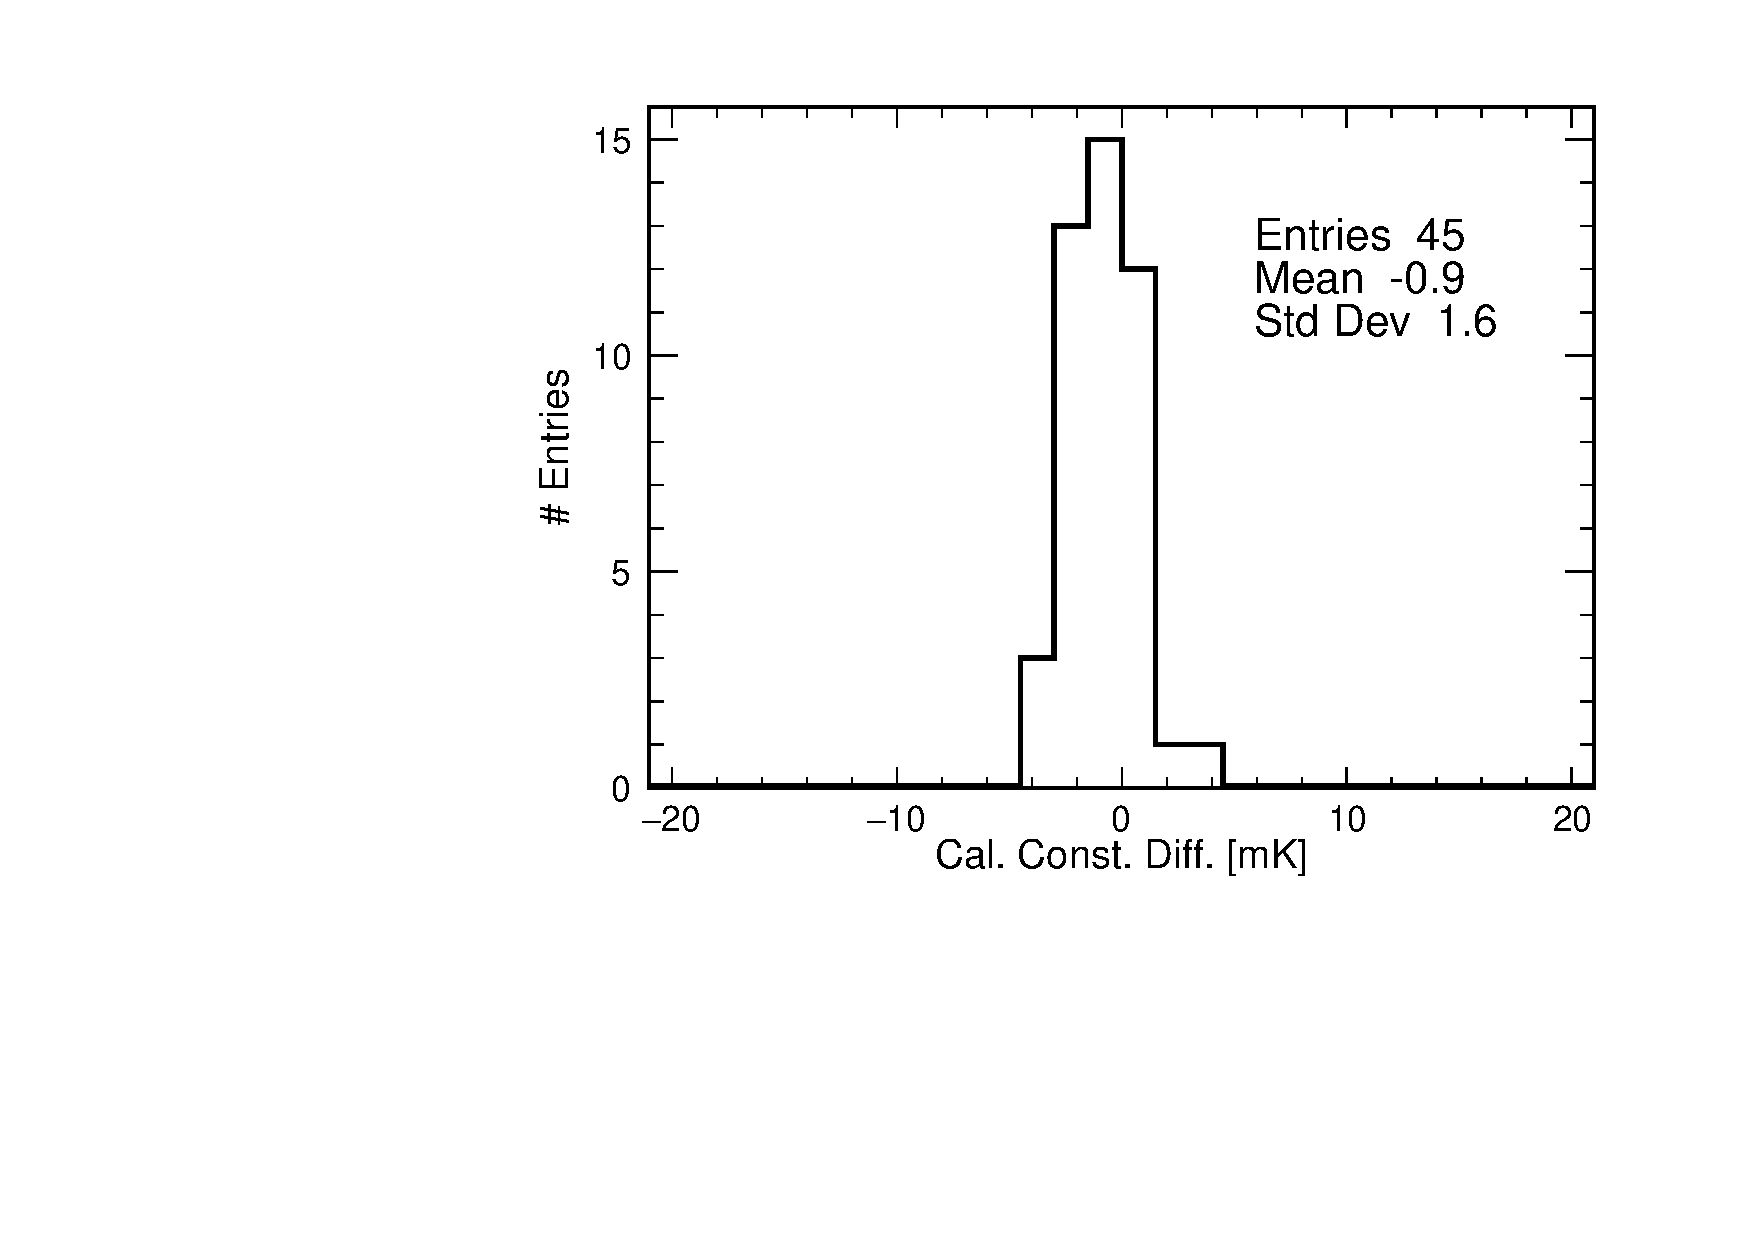
\includegraphics[width=0.32\textwidth]{images/figure_21_a.pdf}}
{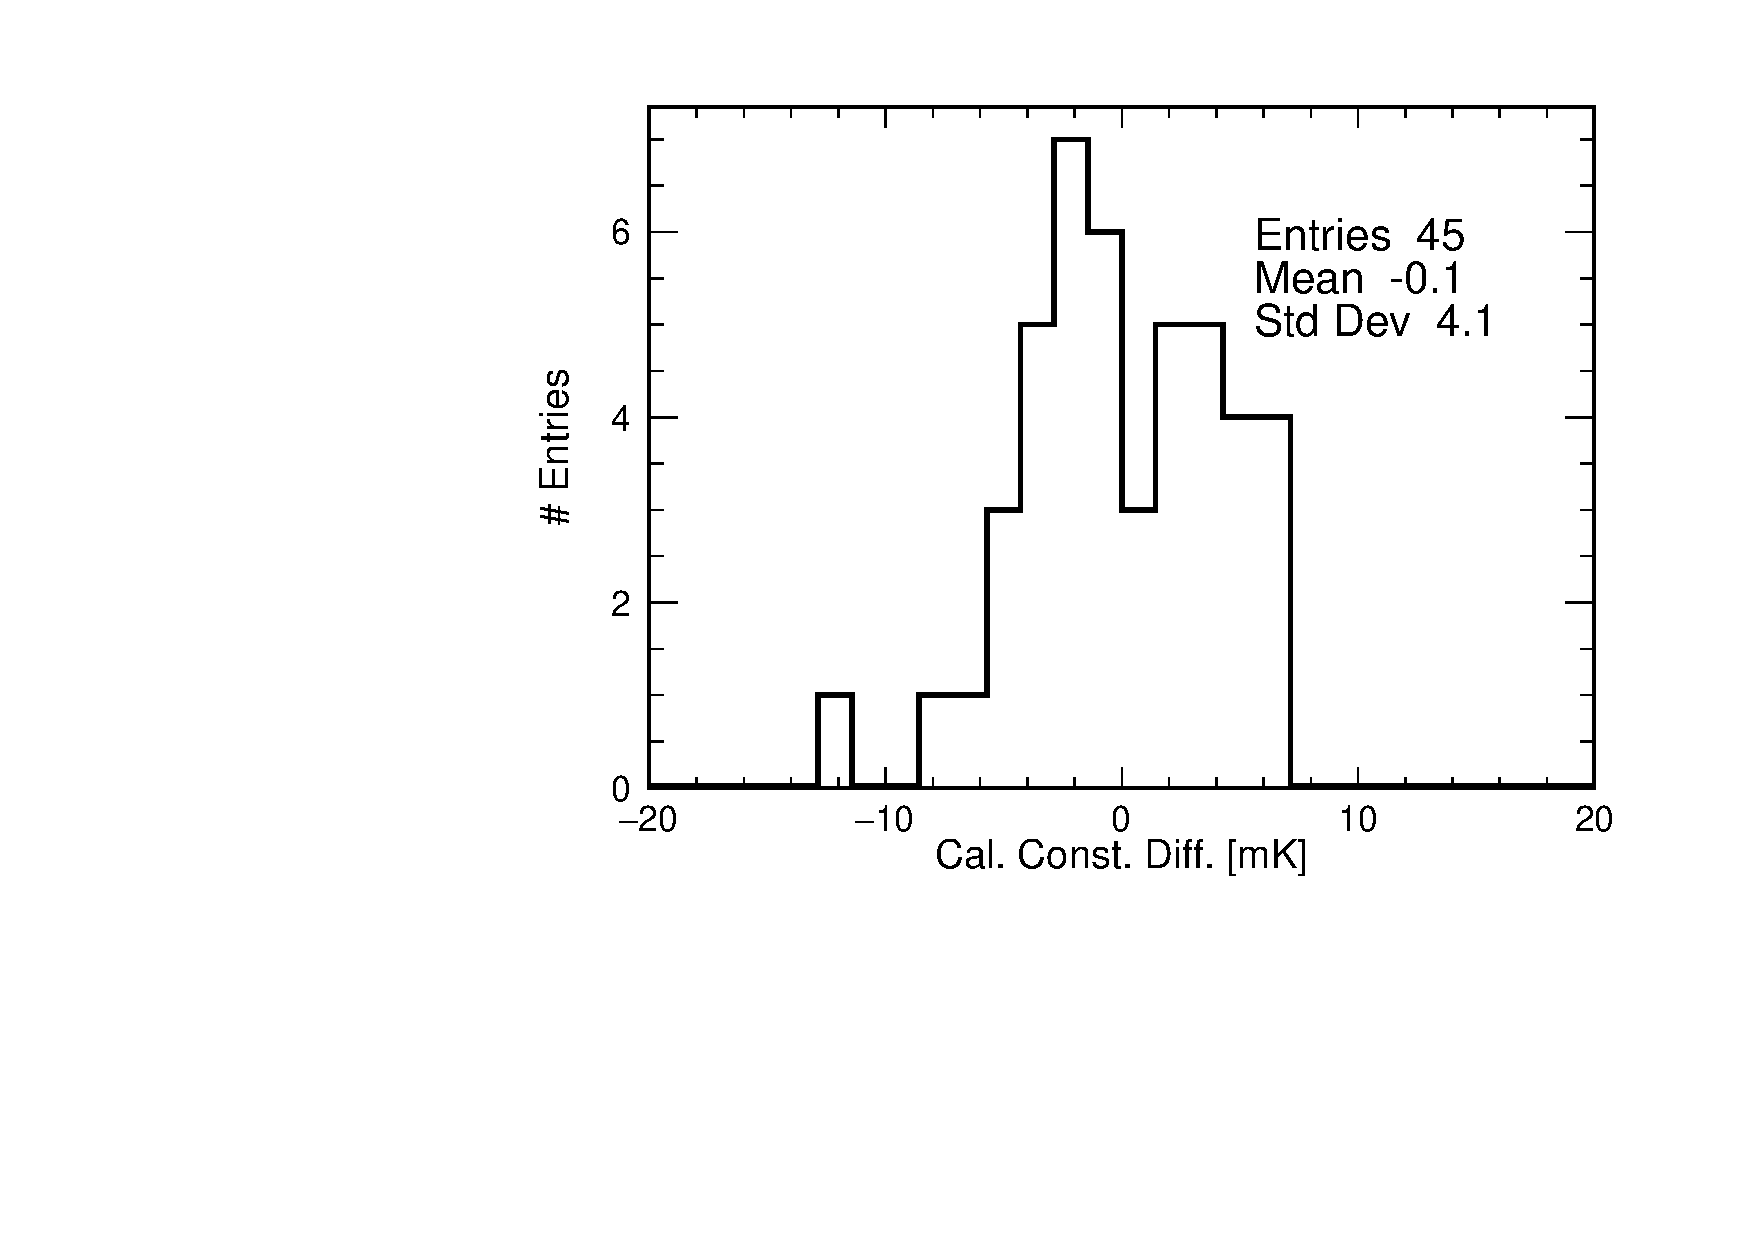
\includegraphics[width=0.32\textwidth]{images/figure_21_b.pdf}}
{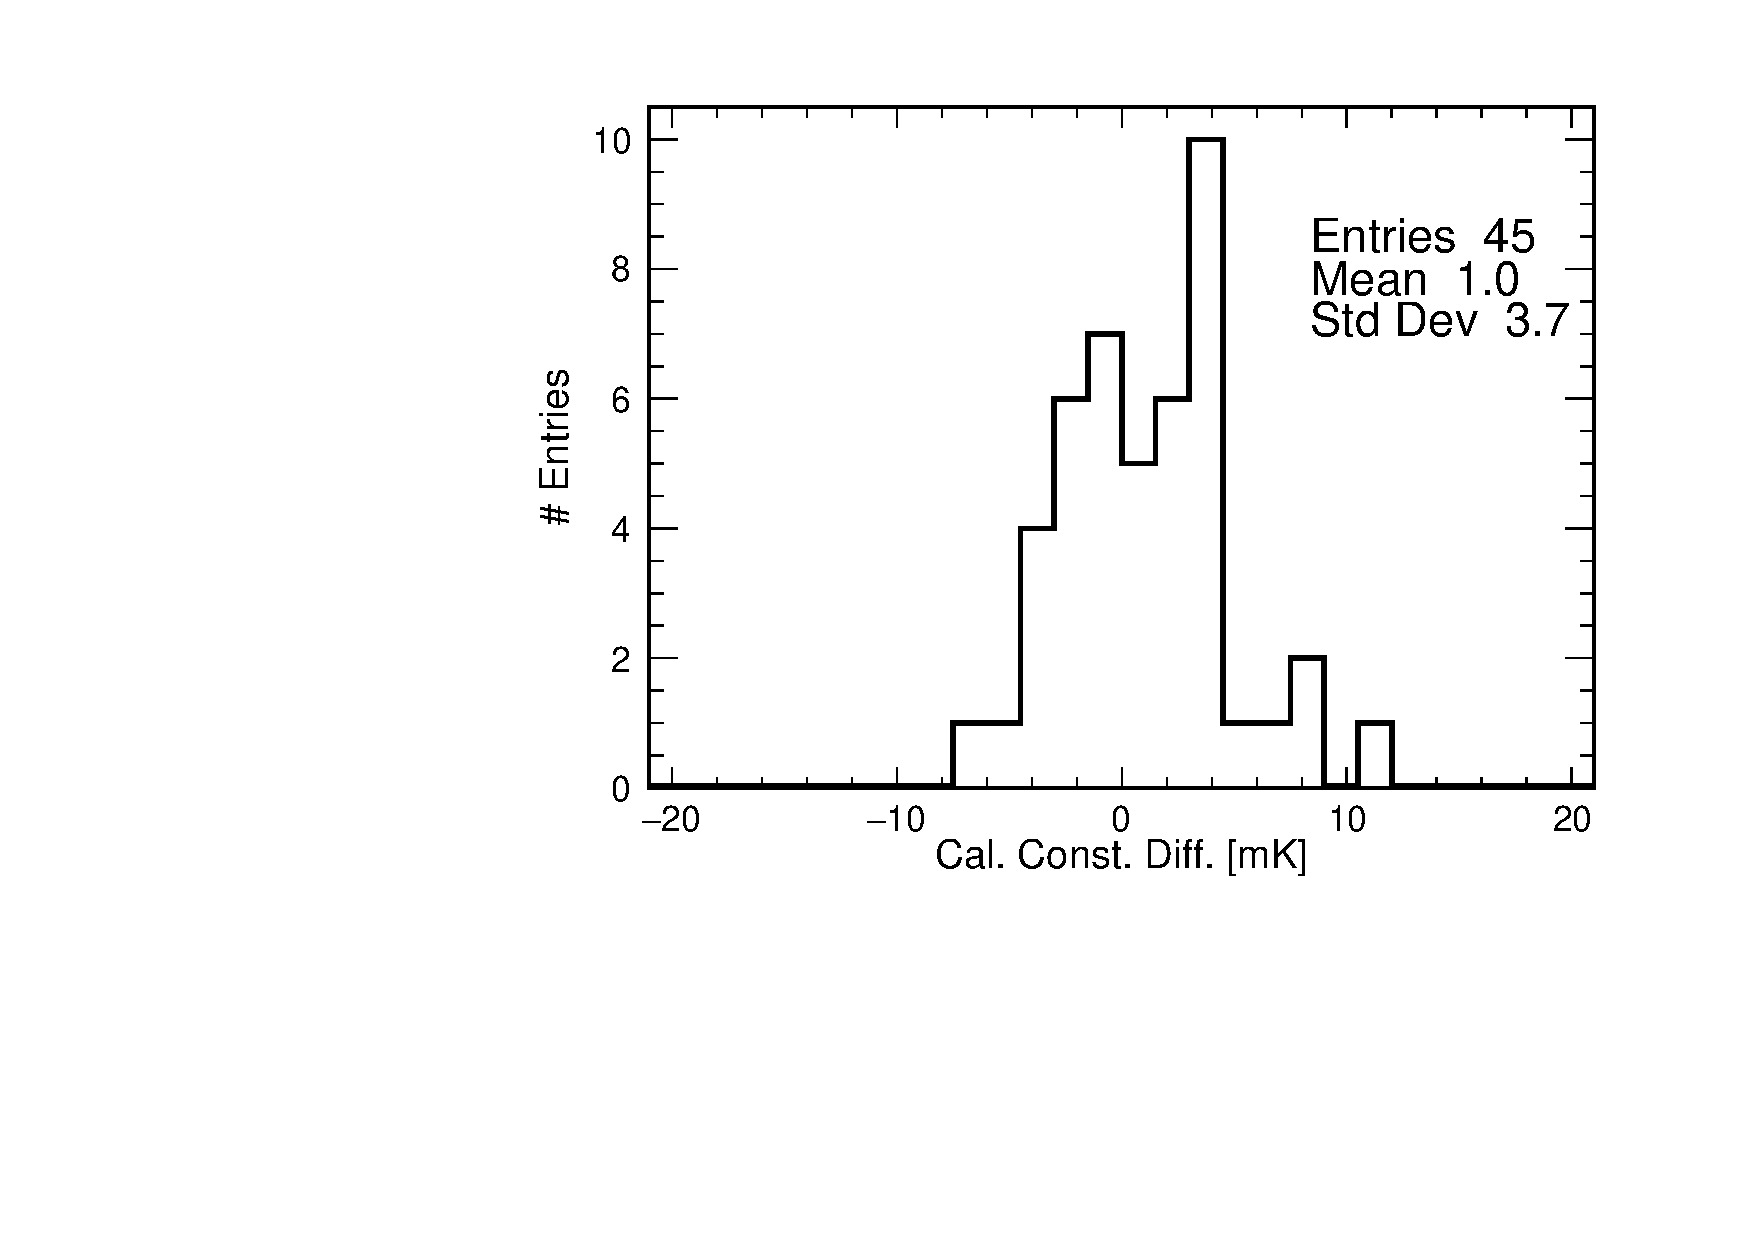
\includegraphics[width=0.32\textwidth]{images/figure_21_c.pdf}}
\caption{Difference between offsets for two calibrations. Left: LN2-2022 and LN2-2023. Middle: LN2-2022 and LAr-2023. Right:  LN2-2023 and LAr-2023.}
\label{fig:comp_newCalib}
\end{figure}

Ageing and long term stability have also been addressed. The left panel of Fig.~\ref{fig:comp_newCalib} shows no difference between the offsets calculated in LN2 with a delay of one year. A better understanding of this effect is achieved by comparing with the LAr-2018 calibration, as shown in the next section.

%------------------------------------------------
\subsection{Comparison between new and old calibrations}
\label{sec:compNewOld}

\noindent Fig. \ref{fig:LAr2018AllDiff} shows the distribution of the offset difference between the LAr-2018 and LAr-2023 calibrations. The mean of the distribution is $-0.1\pm0.6$ mK, excluding any relevant systematic drift. The standard deviation of the distribution, 4.3 mK, is only slightly larger than the ones obtained in the comparison between newer calibrations, which could be due to the unknown contribution of the uncorrected readout offsets, pointing to small or non-existing ageing effects. This can also be observed in Table~\ref{tab:calib_comparison}, summarizing the results of all possible comparisons between calibration campaigns, showing the mean and standard deviation of those comparisons. The lowest standard deviation, 1.6 mK, is obtained for the LN2-2022 to LN2-2023 combination, which is somehow expected since i) the cryogenic liquid is the same, ii) ageing should be small since there is only one year difference and iii) having use the same readout channels, readout offsets cancel out.

\begin{figure}[htbp]
\centering
{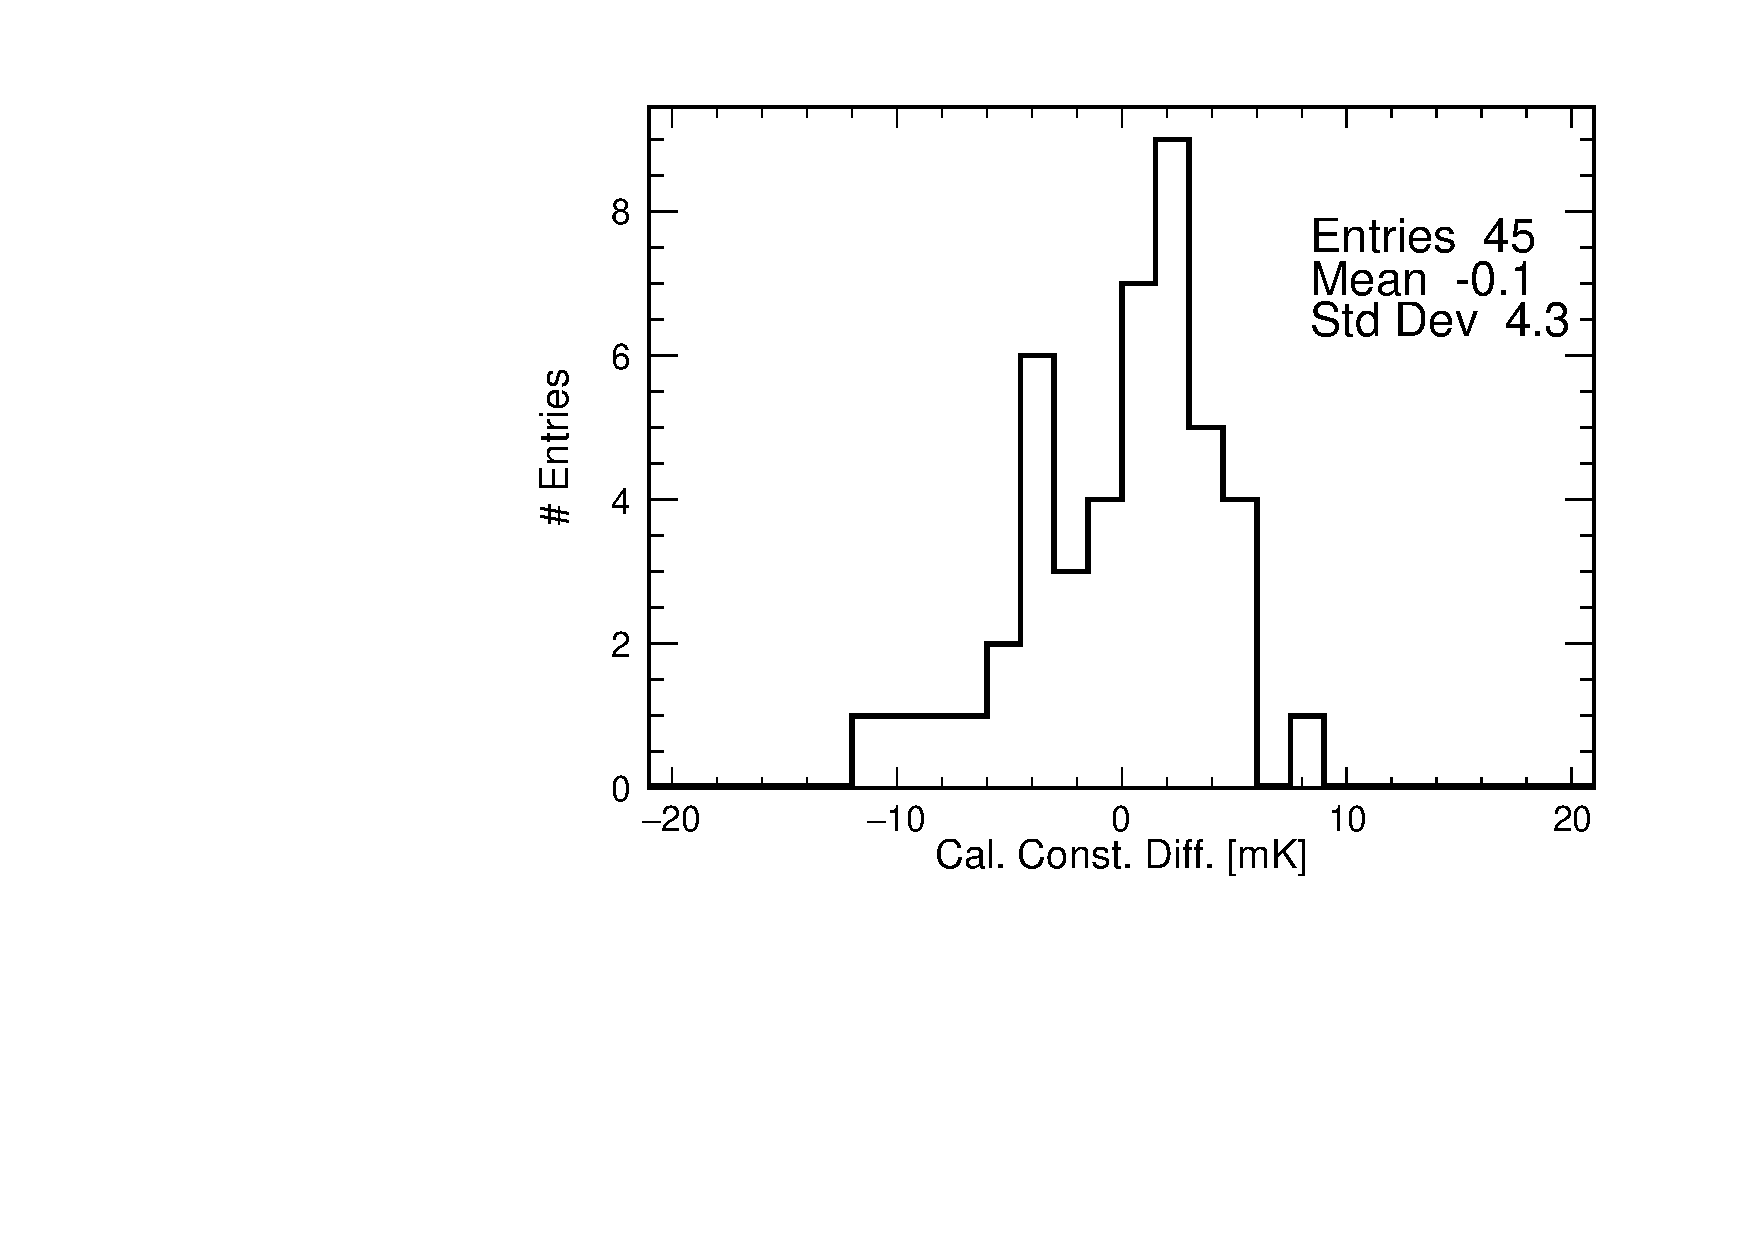
\includegraphics[width=0.65\textwidth]{images/figure_22.pdf}}
\caption{Difference between offsets for LAr-2018 and LAr-2023 calibration campaigns.}
\label{fig:LAr2018AllDiff}
\end{figure}

\begin{table}[htbp]
\begin{center}
\begin{tabular}{l c c c c}
         & LAr-2018 & LN2-2022 & LN2-2023 & LAr-2023  \\ \hline
LAr-2018 &    -     & 0.0, 3.5& 0.9, 3.9 & -0.1, 4.3 \\
LN2-2022 &    -     &    -     & 0.9, 1.6 &  -0.1, 4.1 \\
LN2-2023 &    -     &    -     &    -     & -1.0, 3.7 \\
LAr-2023 &    -     &    -     &    -     &     -     \\
\end{tabular}
\end{center}
\caption{Mean and standard deviation of the difference between the calibration constants obtained in two calibration campaigns.}
\label{tab:calib_comparison}
\end{table}

\noindent The difference between the constants obtained in two calibration campaigns can be used to estimate the total calibration error. Since ProtoDUNE Horizontal Drift (ProtoDUNE-HD), the next iteration of the ProtoDUNE-SP detector, and DUNE will use LAr, the best estimation of the error would come from a LAr to LAr comparison close in time to the actual detector running. Being this combination not available, three other combinations can be used. The comparison between the LN2 calibrations from 2022 and 2023 yields a standard deviation of 1.6~mK, which should represent the quadratic sum of the individual calibration errors. Assuming equal errors for both campaigns, this implies a single calibration error of approximately 1.13~mK. In this case, readout channel offsets cancel out, although real fluctuations in those offsets still contribute to the estimated single calibration error. The comparison between LAr calibrations from 2018 and 2023 provides further insight, with a standard deviation of 4.3~mK, corresponding to a single calibration error of about 3.0~mK. However, this value includes uncorrected readout offsets as well as potential effects from sensor ageing. Finally, comparing the new LAr and LN2 calibration campaigns avoids issues related to readout offsets and ageing but may be affected by the differences in cryogenic liquids. These comparisons yield a similar standard deviation around 3.8~mK, implying a single calibration error of approximately 2.7~mK. This value thus establishes an upper limit on the LAr calibration error. In summary, the individual calibration error in LAr is estimated to lie between 1.6 and 3.0~mK. This range is consistent with an independent estimate of 1.7~mK obtained using a different method for the LAr-2018 calibration (see Sec.~\ref{sec:crossCheck}).


 %The combination (LN2-2022)-(LN2-2023) has a standard deviation of 1.6 mK, which should be the quadratic sum of the the errors of individual calibrations. Assuming this error is the same for both campaigns the single calibration error would be 1.3 mK. In this comparison the readout channel offsets cancel out, but real fluctuations in those offsets contribute to the estimated single calibration error. Comparison between LAr-2018 and LAr-2023 also brings some insights into the single calibration error. The standard deviation is in this case 4.3 mK, corresponding to a single calibration error of 3.0 mK. However, this value includes the uncorrected readout offsets as well as the effect of some potential ageing. Finally, comparison between LAr and LN2 calibrations in the new campaigns, avoids the readout offset and ageing problems, but suffer from potential dependence on the cryogenic liquid. Those comparisons have similar standard deviation of the order of 3.8 mK, corresponding to a single calibration error of 2.7 mK. This figure establishes an upper limit on the LAr calibration error. One can safely conclude that the individual calibration error in LAr is in the range 1.6-3.0 mK. This value is consistent with the one obtained using a different method for the LAr-2018 calibration, 2.4 mK (see Sec.~\ref{sec:crossCheck}).